\documentclass[12pt, dvipsnames]{report}

\usepackage{amsmath}
\usepackage{algorithm}
%\usepackage{algorithmic}
\usepackage[noend]{algpseudocode}

\usepackage{amsmath}
\usepackage{amssymb}
\usepackage{amsthm}
\usepackage{amsopn}

\usepackage{kpfonts}

\usepackage{graphicx}

% Probably don't need this on notes anymore
%\usepackage{kbordermatrix}

% Standard tool for drawing diagrams.
\usepackage{tikz}
\usepackage{tkz-berge}
\usepackage{tikz-cd}
\usepackage{tkz-graph}

\usepackage{comment}

%
\usepackage{multicol}

%
\usepackage{framed}

%
\usepackage{mathtools}

%
\usepackage{float}

%
\usepackage{subfig}

%
\usepackage{wrapfig}

%
\let\savewideparen\wideparen
\let\wideparen\relax
\usepackage{mathabx}
\let\wideparen\savewideparen

% Used for generating `enlightening quotes'
\usepackage{epigraph}

% Forget what this is used for :P
\usepackage[utf8]{inputenc}

% Used for generating quotes.
\usepackage{csquotes}

% Allows what to generate links inside
% generated pdf files
\usepackage{hyperref}

% Allows one to customize theorem
% environments in mathematical proofs.
\usepackage{thmtools}

% Gives access to a proof
\usepackage{lplfitch}

% I forget what this is for.
\usepackage{accents}

% A package for drawing simple trees,
% as a substitute for unnesacary TIKZ code
\usepackage{qtree}

% Enables sequent calculus proofs
\usepackage{ebproof}

% For braket notation
\usepackage{braket}

% To change line spacing when using mathematical notations which require some height!
\usepackage{setspace}

%\usepackage[dvipsnames]{xcolor}

\usepackage{float}

% For block commenting
\usepackage{comment}




\setlength\epigraphwidth{8cm}

\usetikzlibrary{arrows, petri, topaths, decorations.markings}

% So you can do calculations in coordinate specifications
\usetikzlibrary{calc}
\usetikzlibrary{angles}

\theoremstyle{plain}
\newtheorem{theorem}{Theorem}[chapter]
\newtheorem{axiom}{Axiom}
\newtheorem{lemma}[theorem]{Lemma}
\newtheorem{corollary}[theorem]{Corollary}
\newtheorem{prop}[theorem]{Proposition}
\newtheorem{exercise}{Exercise}[chapter]
\newtheorem{fact}{Fact}[chapter]

\newtheorem*{example}{Example}
\newtheorem*{proof*}{Proof}

\theoremstyle{remark}
\newtheorem*{exposition}{Exposition}
\newtheorem*{remark}{Remark}
\newtheorem*{remarks}{Remarks}

\theoremstyle{definition}
\newtheorem*{defi}{Definition}

\usepackage{hyperref}
\hypersetup{
    colorlinks = true,
    linkcolor = black,
}

\usepackage{textgreek}

\makeatletter
\renewcommand*\env@matrix[1][*\c@MaxMatrixCols c]{%
  \hskip -\arraycolsep
  \let\@ifnextchar\new@ifnextchar
  \array{#1}}
\makeatother

\renewcommand*\contentsname{\hfill Table Of Contents \hfill}

\newcommand{\optionalsection}[1]{\section[* #1]{(Important) #1}}
\newcommand{\deriv}[3]{\left. \frac{\partial #1}{\partial #2} \right|_{#3}} % partial derivative involving numerator and denominator.
\newcommand{\lcm}{\operatorname{lcm}}
\newcommand{\im}{\operatorname{im}}
\newcommand{\bint}{\mathbf{Z}}
\newcommand{\gen}[1]{\langle #1 \rangle}

\newcommand{\End}{\operatorname{End}}
\newcommand{\Mor}{\operatorname{Mor}}
\newcommand{\Id}{\operatorname{id}}
\newcommand{\visspace}{\text{\textvisiblespace}}
\newcommand{\Gal}{\text{Gal}}

\newcommand{\xor}{\oplus}
\newcommand{\ft}{\wedge}
\newcommand{\ift}{\vee}

\newcommand{\prob}{\mathbf{P}}
\newcommand{\expect}{\mathbf{E}}
\DeclareMathOperator{\Var}{\mathbf{V}}
\newcommand{\Ber}{\text{Ber}}
\newcommand{\Bin}{\text{Bin}}

%\newcommand{\widecheck}[1]{{#1}^{\ft}}

\DeclareMathOperator{\diam}{\text{diam}}

\DeclareMathOperator{\QQ}{\mathbf{Q}}
\DeclareMathOperator{\ZZ}{\mathbf{Z}}
\DeclareMathOperator{\RR}{\mathbf{R}}
\DeclareMathOperator{\HH}{\mathbf{H}}
\DeclareMathOperator{\CC}{\mathbf{C}}
\DeclareMathOperator{\AB}{\mathbf{A}}
\DeclareMathOperator{\PP}{\mathbf{P}}
\DeclareMathOperator{\MM}{\mathbf{M}}
\DeclareMathOperator{\VV}{\mathbf{V}}
\DeclareMathOperator{\TT}{\mathbf{T}}
\DeclareMathOperator{\LL}{\mathcal{L}}
\DeclareMathOperator{\EE}{\mathbf{E}}
\DeclareMathOperator{\NN}{\mathbf{N}}
\DeclareMathOperator{\DQ}{\mathcal{Q}}
\DeclareMathOperator{\IA}{\mathfrak{a}}
\DeclareMathOperator{\IB}{\mathfrak{b}}
\DeclareMathOperator{\IC}{\mathfrak{c}}
\DeclareMathOperator{\IP}{\mathfrak{p}}
\DeclareMathOperator{\IQ}{\mathfrak{q}}
\DeclareMathOperator{\IM}{\mathfrak{m}}
\DeclareMathOperator{\IN}{\mathfrak{n}}
\DeclareMathOperator{\IK}{\mathfrak{k}}
\DeclareMathOperator{\ord}{\text{ord}}
\DeclareMathOperator{\Ker}{\textsf{Ker}}
\DeclareMathOperator{\Coker}{\textsf{Coker}}
\DeclareMathOperator{\emphcoker}{\emph{coker}}
\DeclareMathOperator{\pp}{\partial}
\DeclareMathOperator{\tr}{\text{tr}}

\DeclareMathOperator{\supp}{\text{supp}}

\DeclareMathOperator{\codim}{\text{codim}}

\DeclareMathOperator{\minkdim}{\dim_{\mathbf{M}}}
\DeclareMathOperator{\hausdim}{\dim_{\mathbf{H}}}
\DeclareMathOperator{\lowminkdim}{\underline{\dim}_{\mathbf{M}}}
\DeclareMathOperator{\upminkdim}{\overline{\dim}_{\mathbf{M}}}
\DeclareMathOperator{\lhdim}{\underline{\dim}_{\mathbf{M}}}
\DeclareMathOperator{\lmbdim}{\underline{\dim}_{\mathbf{MB}}}
\DeclareMathOperator{\packdim}{\text{dim}_{\mathbf{P}}}
\DeclareMathOperator{\fordim}{\dim_{\mathbf{F}}}

\DeclareMathOperator*{\argmax}{arg\,max}
\DeclareMathOperator*{\argmin}{arg\,min}

\DeclareMathOperator{\ssm}{\smallsetminus}

\title{Complex Analysis}
\author{Jacob Denson}

\begin{document}

\pagenumbering{gobble}
\maketitle
\tableofcontents
\pagenumbering{arabic}

\chapter{Introduction}

The study of complex numbers is the analysis of a strange mathematical creation. Originally, these numbers were used as an `imaginary' mathematical creation used to find solutions to polynomial equations. However, in the early 19th century these numbers began being viewed as a geometric construction, another way to describe the two dimensional plane $\mathbf{R}^2$. The introduction of this number system on top of the plane has a much higher structure. And function differentiable with respect to this coordinate system has drastic differences to the study of complex numbers. It offers results many would described as miraculous and magical. What's more, the theory of complex analysis introduces many concepts which have formed the building blocks of many 20th century mathematical fields in topology, geometry, algebra, and analysis. In this first section, we introduce the complex numbers formally, as well as discussing the fundamental tools we will use in the study of complex analysis.

\section{The Complex Numbers}

As a numerical calculation system, the real numbers have many advantages: they are complete, enabling us to use Newton's calculus with precisious, as well as forming an ordered system of numbers, giving us a standard tool for comparing magnitudes which occur throughout the sciences. Nevertheless, the number system has one deficiency: there are some mathematical equations we are unable to solve. Since the square of every real number is positive, we cannot find a number $x$ which satisfies the equation $x^2 = -1$. The complex number system $\mathbf{C}$ is obtained by `imagining' a new number $i$, which does satisfy the equation $i^2 = -1$, and building a new number system containing $i$, and all real numbers, in such a way that most of the useful mathematical laws which hold for the real numbers continue to hold for all numbers in $\mathbf{C}$.

To be precise, we introduce the language of modern algebra. The algebraic rules in $\mathbf{R}$ we tend to use the most often are those which make $\mathbf{R}$ into a {\it field}. We define $\mathbf{C}$ to be the smallest set of numbers containing $\mathbf{R}$, as well as containing a new $i$ satisfying the equation $i^2 = -1$, while also forming a field. Since we must be able to add and multiply arbitrary numbers in $\mathbf{C}$, we must have numbers of the form $a + ib$, for each $a,b \in \mathbf{R}$, because we must be able to multiply each real number by $i$, and to add the result to a real number. Using the commutative and distributive law, we find that
%
\[ (a + ib) + (x + iy) = (a + x) + i(b + y) \]
\[ (a + ib)(x + iy) = (ax - by) + i(bx + ay) \]
%
so the operations of addition and multiplication are closed under these operations. What's more, every nonzero number of the form $z = x + iy$ also has an inverse of this form, because if we define the {\bf complex conjugate} $\overline{z} = x - iy$, we find that $z\overline{z} = x^2 + y^2$, which is a nonzero, positive real number if either $x$ or $y$ is nonzero, and then
%
\[ z \frac{\overline{z}}{x^2 + y^2} = z \left[ \frac{x}{x^2 + y^2} + i \frac{-y}{x^2 + y^2} \right] = 1 \]
%
so the inverse of a complex number $z$ is $\overline{z}(x^2 + y^2)^{-1}$. This means the set of numbers of the form $a + ib$ is precisely the {\it smallest} field containing $\mathbf{R}$ and $i$. Thus every complex number is formally expandable in this form. This expansion must be unique, because if $x + iy = a + ib$, then $(x - a) + i(y-b) = 0$, and if $y \neq b$, we conclude that $i = (a-x)/(y-b)$ is a real number, which is impossible, so we must have $y = b$, and then $x = a$ follows automatically. Thus a complex number $z = a + ib$ is uniquely defined by its real and complex parts $\Re(z) = a$ and $\Im(z) = b$. Summing up these results using the language of field theory, we say that $\mathbf{C}$ is the field extension of degree two obtained from $\mathbf{R}$ by solving the polynomial equation $x^2 = -1$. We also note that since the standard laws of arithmetic apply to the complex numbers, we find that the equations
%
\[ (a + ib) + (x + iy) = (a + x) + i(b + y) \]
\[ (a + ib)(x + iy) = ax + (ay + bx)i + (by)i^2 = (ax - by) + (ay + bx)i \]
%
can be used to formally define the complex numbers; We don't need to `assume' the existence of $\mathbf{C}$ as an axiom. We can instead construct it by placing certain arithmetical operations on $\mathbf{R}^2$, using the definitions above.

Of course, certain properties of the real numbers are lost when we extend to the complex plane. Most importantly, we lose the property of being an ordered field, which was used to define the topological structure of the real line. We cannot possibly give $\mathbf{C}$ an ordered field structure, because in any ordered field we have $x^2 \geq 0$ for all numbers $x$. Nonetheless, in the next section we will show that we can use another algebraic construct to give $\mathbf{C}$ a metric structure by viewing the complex numbers as a `two dimensional' field, whereas the real line is one dimensional.

\section{Geometry of the Complex Plane}

Geometrically, the complex plane can be identified with $\mathbf{R}^2$. This leads to useful insight into the theorems of complex analysis. First off, it gives a topological structure to the class of complex numbers, which when viewed geometrically is called the complex {\it plane}. The $x$ and $y$ axis of the plane are called the {\bf real axis} and {\bf imaginary axis}. A novel result of the introductions of arithmetical operations to $\mathbf{R}^2$ is that the norm has a pleasant form. If we denote the norm of a complex number $z$ by $|z|$, then we have seen that $|z|^2 = x^2 + y^2 = z\overline{z}$, which has a pleasant complex algebraic form. We call $|z|$ the {\bf modulus} of a complex number $z$. Since
%
\[ |zw|^2 = zw \overline{zw} = z\overline{z} w \overline{w} = |z|^2|w|^2 \]
%
we find that $|zw| = |z||w|$ and $|\overline{z}| = |z|$. The modulus gives a complete metric space structure to the complex plane. Just as for the plane, we have the useful inequalities
%
\[ |z+w| \leq |z| + |w|\ \ \ \ \ |\Re(z)|, |\Im(z)| \leq |z|\ \ \ \ \ ||z| - |w|| \leq |z - w| \]
%
which follow from their real analytical theorems about $\mathbf{R}^2$, once converted back to the appropriate language.

Geometrically, the arithmetical operations of the complex numbers become incredibly beautiful when we look at the numbers in their {\bf polar form}. Recall that any point on the plane $\mathbf{R}^2$ can be expressed in terms of an angle $\theta$ and a radius $r$. Looking ahead, we note that the complex exponential $e^{it}$ satisfies Euler's formula $e^{it} = \cos t + i \sin t$ (we will prove this rigorously later), so that is polar coordinates, the number with coordinates $r$ and $\theta$ is exactly $re^{i\theta}$. Because we have the addition formula $e^{i(x + y)} = e^{ix}e^{iy}$, we find that $re^{it}r'e^{it'} = (rr')e^{i(t + t')}$, so that multiplying too complex numbers dilates their radius multiplicatively, and rotates their angular coordinate additively. This means that for any $w \neq 0$, the function $z \mapsto wz$ is a rotation and dilation in two dimensions. In particular, this justifies the utility of the abstractly defined complex numbers; it has a purely geometric definition, which explains why complex analysis leads to such majestic geometrical results, and explains why complex numbers occur in the studies of rotation in physics.

\section{Complex Functions and Holomorphicity}

The really interesting part of complex analysis begin when we start looking at complex-valued functions defined on subsets of the complex plane. Classically, we write such a function in the form $w = f(z)$, referring to the domain as the `$z$-plane', and the codomain as the `$w$-plane'. We will mostly be analyzing maps defined on {\bf domains}, that is, open, connected subsets of the plane. Unless otherwise specified, we will assume that all the domains of the functions we consider are open and connected.
%
%How do we visualize such a function? Is it fairly simple to visualize a real-valued function, defined on a subset of the real numbers, since the graph of such a function lies in two-dimensional space. For complex numbers, it is not so easy to see that the graph approach works, since the graph lies in four dimensional space. We can still analyze pieces of the functions which lie in the real axis. For instance, we can analyze the modulus, argument, real, and imaginary parts of a complex function separately.
%
%A more advanced and very modern way of analyzing a complex function is through {\bf domain colouring}. Via the colour wheel, we may identify every point on the complex plane by a certain colour and intensity. This is the trick which enables us to draw a four-dimensional complex function. At each point $z$, we draw the colour representing $f(z)$. You might not be able to draw this by hand, but if you are able to use a computer, it's a great visual tool.
%
%\begin{example}
%    Consider the function $w = z^2$. If we analyze the graph of the modulus $w = |z^2| = |z|^2$, we see that it is a paraboloid of revolution. The level curves are circles around the origin.
    %
%    \begin{center}
%    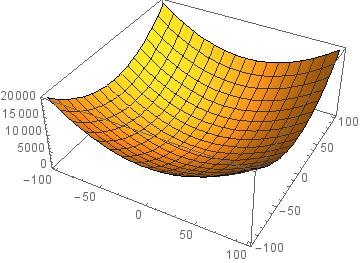
\includegraphics[scale = 0.3]{complexz2abssurface}
%    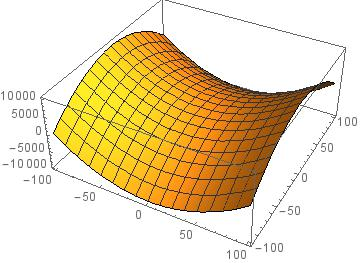
\includegraphics[scale = 0.3]{complexz2resurface}
%    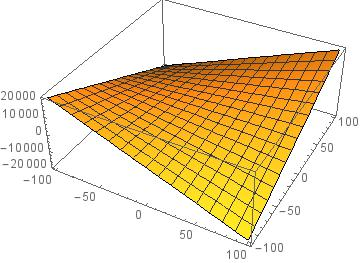
\includegraphics[scale = 0.3]{complexz2imsurface}

%    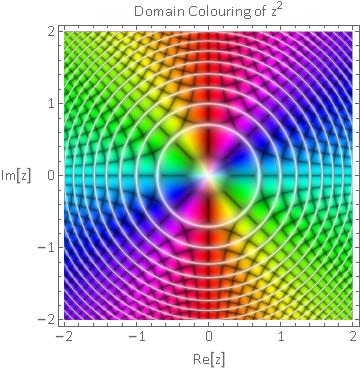
\includegraphics[scale = 0.5]{colorz2}
%    \end{center}
    %
%    The graph of the real part $w = \Re(z^2)$ can be written as $w = \Re(z)^2 - \Im(z)^2$. This is a hyperbololic paraboloid, as is the imaginary part can be written $w = 2\Re(z)\Im(z)$, with level curves
    %
%    \[ \Im(z) = \frac{w}{2 \Re(z)} \]
    %
%    Graphs of the three component functions are shown above.
%\end{example}
%
The standard definition of differentiability of real-valued functions generalizes easily to complex-valued functions, but the definition hides the fact that complex differentiability is a much stronger property than standard differentiability. A complex-valued function $f$ defined in a neighbourhood of a point $z$ = is {\bf complex differentiable}, {\bf holomorphic}, or {\bf regular} at $z$ if the limit
%
\[ f'(z) = \lim_{h \to 0} \frac{f(z + h) - f(z)}{h} \]
%
exists. Unlike differentiability on the real plane, we note that complex differentiability is a much stronger condition on the local behaviour of $f$ around $z$. Whereas the real-valued limit can only by approached by two directions, complex differentiability is a limit approached from any approach trajectory. The set of all holomorphic functions defined on a domain $D$ is denoted $C^\omega(D)$. If $f$ is complex differentiable at $z$, then the limit implies exactly that we can write $f(z + w) = f(z) + w f'(z) + o(w)$. In terms of complex multiplication, that means that $f$ is locally well approximated by a translation, combined with a rotation and a dilation. We leave it to verify that the addition, multiplication, quotient, and chain rule continue to hold from normal calculus, and the proofs are algebraically the same.

\begin{example}
    Every polynomial $f(z) = a_0 + a_1z + \dots + a_nz^n$ is differentiable at any point in the complex plane, with derivative $f'(z) = a_1 + 2a_2z + \dots + na_nz^{n-1}$. It is easy to see that the derivative of $w = z$ is $w' = 1$, and then the addition and product rule verifies the rule for all polynomials.
\end{example}

\begin{example}
    The function $w = 1/z$ is differentiable on $\mathbf{C} - \{ 0 \}$, because
    %
    \[ \lim_{h \to 0} \frac{(z + h)^{-1} - z^{-1}}{h} = \lim_{h \to 0} -\frac{1}{z(z+h)} = -\frac{1}{z^2} \]
    %
    Using the product rule, this implies that for $w = z^{-n}$, $w' = -nz^{-(n+1)}$.
\end{example}

\begin{example}
    The function $f(z) = \overline{z}$, though just a simple reflection in the complex plane, is not {\it complex} differentiable anywhere. This is because
    %
    \[ \lim_{h \to 0} \frac{\overline{z + h} - \overline{z}}{h} = \lim_{h \to 0} \frac{\overline{h}}{h} \]
    %
    And this limit does not exist, because if we approach the limit from the imaginary axis, with $h = ti$, then $\overline{h}/h = -1$, and if we approach the limit from the real axis, with $h = t$, then $\overline{h}/h = 1$. A reflection is not locally a rotation and a dilation.
\end{example}

We previously noted that complex multiplication corresponds to a rotation and a dilation. In particular, for each $w$, the map $T_w(z) = wz$ is a linear map from $\mathbf{C}$ to itself. Viewing $\mathbf{C}$ as $\mathbf{R}^2$, we see it has a matrix representation
%
\[ T_w = \begin{pmatrix} w_1 & w_2 \\ -w_2 & w_1 \end{pmatrix} \]
%
The function $f(z) = \overline{z}$, viewed as a function from $\mathbf{R}^2$ to $\mathbf{R}^2$, is certainly differentiable, and in fact, $C^\infty$. It is linear, with matrix representation
%
\[ \begin{pmatrix} +1 & 0 \\ 0 & -1 \end{pmatrix} \]
%
This cannot be put in the form $T_w$ for any $w$, which reflects the nonexistence of a complex derivative. Not all linear endomorphisms of the plane are homotheties. However, there are relations which guarantee a linear map to be a rotation and a dilation. In fact, the matrix representation above shows that a function $f = u + iv$ is complex differentiable at a point if and only if it is real differentiable, and
%
\[ \frac{\partial u}{\partial x} = \frac{\partial v}{\partial y}\ \ \ \ \ \frac{\partial u}{\partial y} = -\frac{\partial v}{\partial x} \]
%
These are known as the {\bf Cauchy-Riemann equations}. As an alternate viewpoint, we can also approach this purely from the complex perspective, something we will find often gives the most elegant arguments as we go deeper into complex analysis. If $f$ is complex differentiable at $z$, then
%
\[ f(z + w) = f(z) + f'(z)w + o(w) \]
%
so
%
\[ \frac{\partial f}{\partial x} = \lim_{t \to 0} \frac{f(z + t) - f(z)}{t} = \lim_{t \to 0} \frac{f'(z)t + o(t)}{t} = f'(z) \]
\[ \frac{\partial f}{\partial y} = \lim_{t \to 0} \frac{f(z + it) - f(z)}{t} = \lim_{t \to 0} \frac{itf'(z) + o(it)}{t} = if'(z) \]
%
If $f$ is complex differentiable, then we find
%
\[ \frac{\partial f}{\partial y} = i\frac{\partial f}{\partial x} \]
%
This is precisely the Cauchy Riemann equations in complex form.











\section{Power Series}

Polynomials are the simplest examples of holomorphic functions. Our next family of holomorphic functions will be obtained by taking limits of polynomials. In fact, we will soon show that this family essentially contains all holomorphic functions. A {\bf formal power series} about a point $z_0$ is an `infinite dimensional polynomial'
%
\[ \sum_{n = 0}^\infty c_n (z - z_0)^n \]
%
We may evaluate a power series to obtain a function $f$, defined as
%
\[ f(z) = \sum_{k = 0}^\infty a_k (z - z_0)^k \]
%
whose domain is the set where the series converges. A function $f$ can be {\bf expanded in a power series} at a point $z_0$ if we may write $f$ as a power series locally around $z_0$. An {\bf analytic} function is a function which can be locally expanded as a power series at every point in its domain.

Standard tricks from real power series come into play here, and the proofs go unedited. The most useful is the root test, or Cauchy-Hadamard theorem, which states that, if we define
%
\[ 1/R = \limsup_{n \to \infty} |c_n|^{1/n} \]
%
Then the power series $f$ converges locally uniformly for $|z - z_0| < R$, and diverges for $|z - z_0| > R$. It may sometimes be easier to apply the ratio test. If the limit
%
\[ 1/L = \lim_{n \to \infty} \left| \frac{c_{n+1}}{c_n} \right| \]
%
exists, then $f$ converges for $|z - z_0| < L$, and diverges for $|z - z_0| > L$. These statements do not say anything about what happens on the boundary, when $|z - z_0|$ is equal to $R$ or $L$.

\begin{example}
    The most important power series, and perhaps the most important function in mathematics, is the exponential function, defined at all points in the complex plane by the fomrula
    %
    \[ e^z = \exp(z) = \sum_{n = 0}^\infty \frac{z^n}{n!} \]
    %
    Which converges by the ratio test, since $(n+1)!/n! = n \to \infty$. The product formula shows
    %
    \begin{align*}
    \exp(z + w) &= \sum_{k = 0}^\infty \frac{(z + w)^k}{k!} = \sum_{k = 0}^\infty \sum_{j = 0}^k \binom{k}{j} \frac{z^j w^{k-j}}{k!}\\
    &= \sum_{k = 0}^\infty \sum_{j = 0}^k \frac{z^j}{j!} \frac{w^{k-j}}{(k - j)!} = \exp(z) \exp(w)
    \end{align*}
    %
    which gives us the multiplicative property of the function.
\end{example}

\begin{example}
    The hypergeometric series is defined for $\alpha, \beta \in \mathbf{C}$, and $\gamma$ not a negative integer by
    %
    \begin{align*}
        F(\alpha,\beta,\gamma;z) &= \sum_{n = 1}^\infty \frac{\alpha(\alpha+1)\dots(\alpha + n - 1) \beta(\beta + 1) \dots (\beta + n - 1)}{\gamma (\gamma + 1) \dots (\gamma + n - 1)} \frac{z^n}{n!}\\
        &= \sum_{n = 1}^\infty \frac{(\alpha)_n (\beta)_n}{(\gamma)_n} \frac{z^n}{n!}
    \end{align*}
    %
    The notation $(\cdot)_n$ is known as a Pockhammer symbol. We calculate
    %
    \begin{align*}
        \log \left( \prod_{m = 0}^{N-1} (\lambda + m) \right) &= \sum_{m = 0}^{N-1} \log(\lambda + m) = \int_\lambda^{\lambda + N} \log x\; dx + O(\log(\lambda + N))\\
        &= N \log(\lambda + N) + O(\log(\lambda + N))\\
        &= N \log(N) + O(\log(\lambda + N))
    \end{align*}
    %
    In particular, $\log(N!) = N \log N + O(\log N)$. This means
    %
    \[ \log \left( \left( \frac{(\alpha)_n (\beta)_n}{(\lambda)_n} \frac{1}{n!} \right)^{1/n} \right) = \frac{O(\log(\alpha + \beta + \lambda + n))}{n} = o(1) \]
    %
    so
    %
    \[ \left( \frac{(\alpha)_n (\beta)_n}{(\lambda)_n} \frac{1}{n!} \right)^{1/n} \to 1 \]
    %
    so the series has a radius of convergence of one.
\end{example}

\begin{example}
    If we define the Bessel function
    %
    \[ J_m(z) = (z/2)^m \sum_{n = 0}^\infty \frac{(-1)^n}{n! (n+m)!} \]
    %
    Then we calculate
    %
    \begin{align*}
        \log \left( \left( \frac{1}{2^{2n} n! (n+m)!} \right)^{1/2n} \right) &= \frac{-2n \log 2 - 2n \log n + O(\log(n+m))}{2n}\\
        &= - \log 2 - \log n + o(1) \to -\infty
    \end{align*}
    %
    so $J_m$ is defined by a power series everywhere.
\end{example}

Calculus tells us that the derivative of the exponential function is the exponential function itself. If there is any justice in the world, this idea should extend to the complex case. We can formally calculate
%
\[ \exp'(z) = \sum_{n = 0}^\infty \left( \frac{z^n}{n!} \right)' = \sum_{n = 1}^\infty \frac{z^{n-1}}{(n-1)!} = \sum_{n = 0}^\infty \frac{z^n}{n!} = \exp(z) \]
%
But how do we know that the derivative of the power series can be obtained by differentiating each term in the series?

\begin{theorem}
    Let
    %
    \[ f(z) = \sum_{n = 0}^\infty a_n z^n \]
    %
    be a power series, convergent inside a disk $D$. Then $f$ is holomorphic in $D$, and
    %
    \[ f'(z) = \sum_{n = 1}^\infty n a_n z^{n-1} \]
\end{theorem}
\begin{proof}
    The fact that the power series defining $f'$ converges in $D$ follows from the Hadamard formula. Now let us verify that this series, which defines a function $g$, approaches the derivative of $f$. Define $S_n$ to be the finite polynomial of degree $n$ defined by $f$, $S_n(z) = \sum_{k = 0}^n a_k z^k$. Let $E_n$ denote the error term, $E_n(z) = \sum_{k = n+1}^\infty a_k z^k$. Then $S_n'(z) = \sum_{k = 1}^n k a_k z^{k-1}$, and
    %
    \[ \frac{f(z + w) - f(z)}{w} = \left[ \frac{S_n(z + w) - S_n(z)}{w} - S_n'(z) \right] + \left[ \frac{E_n(z + w) - E_n(z)}{w} \right] + S_n'(z) \]
    %
    The first term converges to zero for small enough $w$. The third term converges to $g(z)$ as $n \to \infty$. The only tricky component is the second term. Since $a^n - b^n = (a - b)(a^{n-1} + a^{n-2}b + \dots + ab^{n-2} + b^{n-1})$. If we choose $|z|, |z + w| < r - \varepsilon$, then
    %
    \begin{align*}
        \left| \frac{E_n(z + w) - E_n(z)}{w} \right| &= \left| \sum_{k = n + 1}^\infty a_k \frac{(z + w)^k - z^k}{w} \right| \leq \sum_{k = n + 1}^\infty k |a_k| (r - \varepsilon)^{n-1}
    \end{align*}
    %
    The right side is a convergent power series, and hence as $n \to \infty$, the term converges to zero. By picking $n$ large enough, and $|z - w|$ small enough, the value can be made as close to $g$ as possible.
\end{proof}

\begin{corollary}
    The power series $f$ is infinitely differentiable in $D$, with
    %
    \[ f^{(m)}(z) = \sum_{n = m}^\infty \frac{n!}{(n - m)!} a_n z^{n-m} \]
\end{corollary}
\begin{proof}
    All that remains to be proven is that $f'$ has the same radius of convergence as $f$, so that we may successively apply the theorem. If $f$ has radius of converge $R$, then $R^{-1} = \limsup |a_n|^{1/n}$, and so
    %
    \[ \limsup |a_n|^{1/n} n^{1/n} = \lim n^{1/n} \limsup |a_n|^{1/n} = \limsup |a_n|^{1/n} \]
    %
    and so $f'$ has the same radius of convergence as $f$.
\end{proof}

\begin{corollary}
    Every analytic function is holomorphic throughout it's domain.
\end{corollary}











\section{Integration Along Curves}

One distinguishing feature separating the study of complex analysis from Newton's one dimensional calculus is the reliance on line integration, which you may have encountered in multivariate calculus. Firstly, we will find ourselves not integrating over the whole complex plane, but instead integrating over curves lying in the complex plane. A {\bf smooth curve} is an immersion of a closed interval into $\mathbf{C}$ (viewing the interval as an oriented one dimensional manifold with boundary, and $\mathbf{C}$ as a two dimensional manifold). More simply, we define a {\bf smooth parameterization} $z: [a,b] \to \mathbf{C}$ to be a differentiable map whose derivative is continuous, and $z'(t) \neq 0$ for all $t \in [a,b]$, where we interpret $z'(a)$ and $z'(b)$ as the left and right hand limits
%
\[ \lim_{h \to 0^+} \frac{z(a + h) - z(a)}{h}\ \ \ \ \ \lim_{h \to 0^-} \frac{z(b + h) - z(b)}{h} \]
%
Two smooth curves $z_0: [a_0,b_0] \to \mathbf{C}$ and $z_1: [a_1,b_1] \to \mathbf{C}$ are {\bf equivalent} if there is a continuously differentiable function $s: [a_0,b_0] \to [a_1,b_1]$ with $s'(t) > 0$ for all $t$, such that $z_0(t) = z_1(s(t))$ for all $t \in [a_0,b_0]$. We then define a smooth curve to be an equivalence class of smooth parameterizations. More generally, a {\bf piecewise smooth curve} is an equivalence class of continuous parameterizations $z: [a,b] \to \mathbf{C}$, with values $a = a_0 < a_1 < \dots < a_n = b$ such that $z$ is a smooth curve on $[a_i,a_{i+1}]$, where $z_0: [a_0,b_0] \to \mathbf{C}$ and $z_1:[c_0,d_0] \to \mathbf{C}$ are equivalent if there are $a = a_0 < \dots < a_n = b$ and $c = c_0 < \dots < b_n = d$ such that $z_0$ and $z_1$ are equivalent on each of the intervals $[a_i,a_{i+1}]$ and $[c_i,c_{i+1}]$. We rarely need to discuss classes of curves more general than this in complex analysis, and certainly not in elementary complex analysis.

\begin{example}
    The standard example of a curve is the circle $C_r(z_0)$, of radius $r$ centered at $z_0$. The {\it positive orientation} of this curve is given by the parameterization
    %
    \[ z(t) = z_0 + re^{it} \]
    %
    On $[0,2\pi]$, and the {\it negative orientation}
    %
    \[ z(t) = z_0 + re^{-it} \]
    %
    also defined on $[0,2\pi]$. In general, we will interpret $C_r(z_0)$ as having the positive orientation. In particular, we denote $C_1(0)$ by $S^1$, the unit circle.
\end{example}

We will also need to introduce slightly more terminology to manipulate curves. The {\bf trace} of a curve $C$ is the point set corresponding to the curve. It is the image of all the parameterizations of the curve. The {\bf inverse orientation} of a curve with parameterization $z: [a,b] \to \mathbf{C}$, which is the curve with parameterization $z^-: [a,b] \to \mathbf{C}$ with $z^-(t) = z(a+b-t)$. A curve $z: [a,b] \to \mathbf{C}$ is {\bf closed} if $z(a) = z(b)$, which means its image forms a `closed loop' in the plane. Now given a smooth curve $C$ with parameterization $z: [a,b] \to \mathbf{C}$, and a continuous function defined on the trace of $C$, we define the {\bf line integral} of $f$ on $C$ as
%
\[ \int_C f(z) dz = \int_a^b f(z(t)) z'(t) dt \]
%
which we can remember by the mneumonic
%
\[ f(z) dz = f(z) \left( \frac{dz}{dt} \right) dt \]
%
so we can obtain the formula by `multiplying by a $dt/dt$ factor'. If $z'$ is only piecewise smooth, with partition $a_0 < \dots < a_n$, then we define
%
\[ \int_C f(z) dz = \sum \int_{a_i}^{a_{i+1}} f(z(t)) z'(t) dt \]
%
The change of variables formula for one dimensional integrals verifies that these definitions are independent of parameterization.

\begin{theorem}
    The line integral satisfies the following properties
    %
    \begin{itemize}
        \item For a given curve $C$ on some domain $D$, for any two $f,g \in C(D)$, $\alpha, \beta \in \mathbf{C}$,
        %
        \[ \int_C (\alpha f + \beta g)(z) dz = \alpha \int_C f(z) dz + \beta \int_C g(z) dz \]

        \item If $C^-$ is the reverse orientation of $C$, then
        %
        \[ \int_{C^-} f(z) dz = - \int_C f(z) dz \]

        \item One has
        %
        \[ \left| \int_C f(z) dz \right| \leq l(C) \| f \|_\infty \]
        %
        where $\| f \|_\infty$ is the supremum of $f$ over image of the curve $C$, and $l(C)$ is the {\bf length} of the curve $C$, defined to be the integral $\int_a^b |z'(t)| dt$.
    \end{itemize}
\end{theorem}
\begin{proof}
    The first theorem follows by the linearity of one dimensional integration by expanding out formulas, and the second theorem follows because $(z^-)'(t) = -z'(a+b-t)$. Finally, the third theorem follows because if $z: [a,b] \to \mathbf{C}$ is smooth, then
    %
    \[ \left| \int_C f(z)dz \right| = \left| \int_a^b f(z(t)) z'(t) dt \right| \leq \int_a^b |f(z(t))||z'(t)| dt \leq \| f \|_\infty \int_a^b |z'(t)| dt \]
    %
    and the result for piecewise smooth curves follows by linearity.
\end{proof}

Finally in our review of line integration, we recall a very useful result. We say a function $f: D \to \mathbf{C}$ on some domain $D$ has a {\bf primitive} if there is a function $F: D \to \mathbf{C}$ holomorphic on $D$ such that $F'(z) = f(z)$.

\begin{theorem}
    If $f$ is continuous, and has a primitive $F$, then a curve $C$ begining at $z_0$ and ending at $z_1$ has
    %
    \[ \int_C f(z)dz = F(z_1) - F(z_0) \]
    %
    In particular, if $C$ is a closed curve, then $\int_C f(z)dz = 0$.
\end{theorem}
\begin{proof}
    If $C$ is smooth, then
    %
    \[ \int_C f(z)dz = \int_a^b f(z(t)) z'(t) dt \]
    %
    Now if $F'(z) = f(z)$ for each $z \in D$, then the chain rule (which is easily proved for compositions of functions from intervals to $\mathbf{C}$ and from holomorphic functions on $\mathbf{C}$) implies that $(F \circ z)'(t) = F'(z(t)) z'(t)$, and therefore the fundamental theorem of calculus (applied componentwise on the integral of the complex valued function $f(z(t)) z'(t)$), we conclude that
    %
    \[ \int_a^b f(z(t)) z'(t) dt = F(z(b)) - F(z(a)) = F(w) - F(z) \]
    %
    The theorem is then proved for piecewise smooth curves by applying this theorem for the individual smooth curves and then applying a telescoping summation.
\end{proof}

\begin{corollary}
    If $f$ is holomorphic, with $f' = 0$, then $f$ is constant on $D$.
\end{corollary}
\begin{proof}
    If $z_0$ and $z_1$ are two points, let $C$ be a smooth curve beginning at $z_0$ and ending at $z_1$. Then since $f' = 0$,
    %
    \[ \int_C f'(z) dz = 0  \]
    %
    But also since $f'$ has a primitive $f$, we find that
    %
    \[ \int_C f'(z) dz = f(z_1) - f(z_0) \]
    %
    and hence $f(z_0) = f(z_1)$.
\end{proof}

\begin{example}
    The function $f(z) = 1/z$ does not have a primitive in $\mathbf{C} - \{ 0 \}$, where it is defined, because
    %
    \[ \int_{S^1} \frac{dz}{z} = \int_0^{2\pi} \frac{ie^{it}}{e^{it}} = \int_0^{2\pi} i = 2 \pi i \]
    %
    If $1/z$ did have a primitive, we would conclude this integral is zero. We shall find that this is the essential holomorphic function without a primitive, and we will use this theorem to calculate a great many contour integrals.
\end{example}

We know that if $f$ has a primitive $F$, then $\int_\gamma f(z)\; dz = 0$ for all closed curves $\gamma$. But conversely, if $\int_\gamma f(z)\; dz = 0$ for all closed curves $\gamma$, then such a primitive exists. The idea is to fix a point $z_0$ in the domain, and to define $F(z_1) = \int_\gamma f(z)\; dz$, where $\gamma$ is a curve from $z_0$ to $z_1$. We find that
%
\[ \frac{\partial F}{\partial x} = f(z)\ \ \ \ \ \frac{\partial F}{\partial y} = i f(z) \]
%
follows from the fundamental theorem of calculus. But this implies that $F$ is holomorphic by the Cauchy Riemann equations, and the continuity of $f$, and $F' = f$.







\section{Harmonic Functions}

A function $f: \mathbf{R}^2 \to \mathbf{C}$ is known as harmonic if
%
\[ \Delta f = \frac{\partial^2 f}{\partial x^2} + \frac{\partial^2 f}{\partial y^2} = 0 \]
%
We now discuss a connection which allows us to reduce their study to the study of holomorphic functions. We calculate
%
\[ \partial_z \partial_{\overline{z}} = \frac{(\partial_x - i \partial_y)(\partial_x + i \partial_y)}{4} = \frac{\partial^2_x + i \partial_x \partial_y - i \partial_y \partial_x + \partial_y^2}{4} = \frac{\Delta}{4} \]
%
So any holomorphic or antiholomorphic function is harmonic, as is it's real and imaginary part. Conversely, suppose that $g$ is a real-valued harmonic function. Then $\partial_{\overline{z}} \partial_z g = 0$, so $\partial_z g$ is holomorphic. We will later find that any holomorphic locally has an antiderivative, so in particular, we can find a holomorphic function $f$ with $f' = 2 \partial_z g$. But this means that
%
\[ \partial_x f_0 - i \partial_y f_0 = f' = 2 \partial_z g = \partial_x g - i \partial_y g \]
%
so $\nabla f_0 = \nabla g$, implying $f_0$ and $g$ differ by a constant. Patching the $f_0$ together shows that $g$ is the real part of a holomorphic function.

In particular, this implies that for any circle $C_r(z_0)$,
%
\[ 2 \pi i f(z_0) = \int_{C_r(z_0)} \frac{f(z)}{z - z_0}\; dz = i \int_0^{2\pi} f(z_0 + r e^{it})\; dt  \]
%
Taking the imaginary parts on both sides gives
%
\[ 2 \pi g(z_0) = \int_0^{2\pi} f(z_0 + e^{it})\; dt \]
%
So any harmonic function satisfies the mean value formula; the average value of the function around a circle is the same as the value of that function at the centre of the circle. Note that this is not necessarily true for the average of the function over every curve, since in the calculations above for curves other than circles the imaginary parts of $f$ might contribute to the imaginary part of the integral.







\chapter{Cauchy's Theorem}

Cauchy's theorem says that the integral of a holomorphic function about a closed curve is always zero. This is simple, but forms the backbone for the theory of holomorphic functions. Originally, certain regularity were assumed on holomorphic functions to obtain Cauchy's theorem. But it was later discovered that one can obtain Cauchy's theorem assuming only that the function is holomorphic at each point in the region, and it is this procedure we will use to show the regularity of holomorphic functions completely.

\begin{theorem}[Goursat's lemma]
    If $T$ is a triangle, and $f$ is holomorphic in an open set containing the triangle and it's interior, then
    %
    \[ \int_T f(z)\; dz = 0 \]
\end{theorem}
\begin{proof}
    We can split the triangle $T$ into four smaller triangles $A$, $B$, $C$, and $D$, each with half the diameter and length. Since
    %
    \[ \int_T f(z)\; dz = \left( \int_{A} f(z)\; dz + \int_B f(z)\; dz + \int_C f(z)\; dz + \int_D f(z)\; dz \right) \]
    %
    We may choose one such triangle $T_1$ with
    %
    \[ \left| \int_{T_1} f(z)\; dz \right| \geq \left| \int_T f(z)\; dz \right| \]
    %
    Continuing inductively, we can find a nested family of rectangles $T_1 \supset T_2 \supset \dots T_n$ with $\text{diam}(T_n) = \text{diam}(T)/2^n$, $l(T_n) = l(T)/2^n$, and
    %
    \[ \left| \int_{T_n} f(z)\; dz \right| \geq 4^{-n} \left| \int_T f(z)\; dz \right| \]
    %
    As $n \to \infty$, $\text{diam}(T_n) \to 0$, so $\bigcap T_n$ contains a unique point $z_0$. We can write $f(z) = f(z_0) + f'(z_0) (z - z_0) + \psi(z - z_0)(z - z_0)$, with $\psi(w) \to 0$ as $w \to 0$. Now it is easy to calculate that
    %
    \[ \int_{T_n} f(z_0)\; dz = f'(z_0) \int_{T_n} (z - z_0)\; dz = 0 \]
    %
    so if $|\psi(z - z_0)| \leq \varepsilon$ for $z$ lying on $T_n$,
    %
    \begin{align*}
        \left| \int_T f(z)\; dz \right| \leq 4^n \left| \int_{T_n} f(z)\; dz \right| &= 4^n \left| \int_{T_n} \psi(z-z_0)(z - z_0)\; dz \right|\\
        &\leq 4^n \varepsilon l(T_n) \text{diam}(T_n) = \varepsilon l(T) \text{diam}(T)
    \end{align*}
    %
    and thus as $n \to \infty$, we can take $\varepsilon \to 0$ to conclude the integral over the triangle is zero.
\end{proof}

\begin{remark}
    Note that the proof of this theorem remains true if we replace the condition that $f$ is holomorphic in $D$ with the weaker condition that $f$ is analytic except at finitely many points $z_1, \dots, z_N$ in the interior of the triangle, with the property that $\lim_{z \to z_n} (z - z_n) f(z) = 0$ for each $n$. By splitting our triangles into smaller triangles, we may assume that there is only a single point with this property in the triangle. By splitting our triangle into smaller triangles, and applying the theorem above in all regions but the region containing the triangle, we determine that the integral over the entire region is equal to the integral of $f$ about an equilateral triangle $T'$ centered at $z$, of arbitrarily small length. But if $T'$ is small enough that $|z - z_n| |f(z)| \leq \varepsilon$ for $z$ on $T'$, then
    %
    \[ \left| \int_{T'} f(z)\; dz \right| \leq \varepsilon \left| \int_{T'} \frac{dz}{z - z_n} \right| \]
    %
    and one verifies that
    %
    \[ \left| \int_{T'} \frac{dz}{z - z_n} \right| \lesssim 1 \]
    %
    since the distance from points on the triangle to $z_n$ is proportional to the perimeter of the triangle. This concludes the argument.
\end{remark}

Attaching two triangles together, we can obtain Cauchy's theorem for a rectangle. Given a holomorphic function $f$ on a circle, by defining $F(w)$ to be the line integral from the centre of the circle to $w$ on either half of the rectangle parallel to the axis, we find a function $F$ with $F' = f$, so $f$ has a primitive, and so Cauchy's theorem holds in a circle. More generally, this holds under the weaker condition where $f$ is defined except at finitely many interior points $z_1, \dots, z_N$ with $\lim (z - z_n) f(z) = 0$, because we can with a few edge cases not included in the previous case find a function $F$ with $F' = f$.

\begin{lemma}
    If $\gamma$ is a closed curve not passing through $z_0$, then
    %
    \[ \eta(\gamma,z_0) = \frac{1}{2 \pi i} \int_\gamma \frac{dz}{z - z_0} \]
    %
    is an integer, known as the {\bf winding number} of $\gamma$ around $z_0$.
\end{lemma}
\begin{proof}
    If we parameterize $\gamma$ by $z$, then consider the continuous function
    %
    \[ h(t) = \int_a^t \frac{z'(t)}{z(t) - z_0}\; dt \]
    %
    And we have $h'(t) = z'(t)/(z(t) - z_0)$. Thus the derivative of $g(t) = e^{-h(t)}(z(t) - z_0)$ vanishes, so $g(t)$ must be constant, so
    %
    \[ e^{h(t)} = \frac{z(t) - z_0}{z(a) - z_0} \]
    %
    In particular,
    %
    \[ e^{h(b)} = \frac{z(b) - z_0}{z(a) - z_0} = 1 \]
    %
    so $h(b)$ must be a multiple of $2 \pi i$, completing the proof.
\end{proof}

Cauchy's theorem implies that if $\gamma$ is contained in a circle, and $z_0$ is a point lying outside of the circle, then $\eta(\gamma,z_0) = 0$. Furthermore, if there is a curve between two points $z_0$ and $z_1$ not passing through $\gamma$, then $\eta(\gamma,z_0) = \eta(\gamma,z_1)$. Since we can replace the curve with a polygon, it suffices to prove this assuming the curve is a line segment. Outside of the segment the function $(z - z_0)(z - z_1)^{-1}$ is never a negative number, so $\log((z-z_0)/(z-z_1))$ is analytic in the complement of the segment, and it's derivative is $(z - z_0)^{-1} - (z - z_1)^{-1}$, hence Cauchy's theorem implies that
%
\[ \int_\gamma \frac{dz}{z - z_0} = \int_\gamma \frac{dz}{z - z_1} \]
%
hence $\eta(\gamma,z_0) = \eta(\gamma,z_1)$.

\begin{theorem}
    If $f$ is holomorphic in a disc $D$ containing a point $w$, and $\gamma$ is a closed curve in $D$ not passing through $w$, then
    %
    \[ \int_\gamma \frac{f(z)}{z - w} = 2 \pi i \eta(\gamma,w) f(w) \]
\end{theorem}
\begin{proof}
    Since $g(z) = (f(z) - f(w))/(z-w)$ is holomorphic everywhere in $D$ except at $w$, and $\lim_{z \to w} (z - w) g(z) = 0$, we can apply our remark to conclude that
    %
    \[ \int_\gamma \frac{f(z)}{z - w}\; dz = \int_\gamma \frac{f(w)}{z - w}\; dz = 2 \pi i \eta(\gamma,w) f(w) \]
    %
    Thus the theorem becomes an explicit calculation.
\end{proof}

\begin{remark}
Integral representation formulas are very important in analysis, because they enable us to control a function from its behaviour on a very small set, and also use it to show the function is suitably regular.
\end{remark}

\section{Consequences of Cauchy's Formula}

A simple corollary of Cauchy's integral formula, proved by induction, shows any holomorphic function is completely smooth.

\begin{theorem}
    If $f$ is holomorphic, then $f$ has derivatives of all orders, with
    %
    \[ f^{(n)}(w) = \frac{n!}{2 \pi i \eta(\gamma,w)} \int_\gamma \frac{f(z)}{(z - w)^{n+1}}\; dz \]
    %
    where $\gamma$ is some closed curve with nonzero winding number obout $w$.
\end{theorem}
\begin{proof}
    To prove this, it would suffice to reduce the question to the theory of differentiation under the integral sign in real variable theory. But there is a more elementary proof. We know this is true for $n = 0$. And now by induction, if it is true for $n$, then
    %
    \begin{align*}
        \frac{n!}{2 \pi i \eta(\gamma,w)} \int_\gamma & \left( \frac{f(z)}{(z - w)^{n+1}} - \frac{f(z)}{(z - w_0)^{n+1}} \right)\; dz\\
        &= \frac{n!}{2 \pi i \eta(\gamma,w)} \int_\gamma \frac{f(z)}{w_0 - w} \left( \frac{1}{z - w} - \frac{1}{z - w_0} \right) \left( \sum_{k = 0}^n \frac{1}{(z - w)^{n-k}(z - w_0)^k} \right)\\
        &= \frac{n!}{2 \pi i \eta(\gamma,w)} \int_\gamma \frac{f(z)}{(z - w)(z - w_0)} \left( \sum_{k = 0}^n \frac{1}{(z - w)^{n-k}(z - w_0)^k} \right)
    \end{align*}
    %
    and as $w \to w_0$, we conclude that
    %
    \[ f^{(n+1)}(w_0) = \frac{(n+1)!}{2 \pi i \eta(\gamma,w)} \int_\gamma \frac{f(z)}{(z - w_0)^{n+2}}\; dz \]
    %
    which completes the proof.
\end{proof}

\begin{remark}
    Because of this, we obtain that for each $z$ upon which $f$ is holomorphic,
    %
    \[ \| f^{(n)}(z) \| \leq \frac{n!}{2\pi \eta(\gamma,z)} \frac{\| f \|_{L^\infty(\gamma)}}{d(z,\gamma)^n} l(\gamma) \]
    %
    a result known as Cauchy's inequality. In the case that $\gamma$ is just a disk centered at $z$ with radius $R$, the formula simplifies to
    %
    \[ \| f^{(n)}(z) \| \leq n! \frac{\| f \|_{L^\infty(\gamma)}}{R^n} \]
\end{remark}

Another regularity property enables us to show every holomorphic function is analytic, because
%
\[ \frac{1}{z - w} = \frac{1}{(z - z_0 - (w - z_0))} = \sum_{n = 0}^\infty \frac{(w - z_0)^n}{(z - z_0)^{n+1}} \]
%
which converges uniformly on $\partial D$, hence we can interchange integration and summation in Cauchy's integral formula to obtain a power series representation of $f$ from Cauchy's integral formula. For the next theorem, one needs to know that an {\bf entire} function is one which is holomorphic on the entire complex plane.

\begin{theorem}[Louville]
    Every bounded and entire function is constant.
\end{theorem}
\begin{proof}
    Consider Cauchy's inequality for $n = 1$, which we just proved. As we take the radius of the disc $D$ to $\infty$, the term $\| f \|_{L^\infty(\partial D)}$ remains bounded, so the numerator is bounded, whereas the denominator tends to $\infty$ for every $z$. Thus we conclude $f' = 0$, so $f$ is constant.
\end{proof}

\begin{theorem}[The Fundamental Theorem of Algebra]
    Every nonconstant polynomial over the complex numbers has a root.
\end{theorem}
\begin{proof}
    Let $f$ be a polynomial with no root over the complex numbers. If $f$ has degree $n$, then for large $z$, $f(z) = (1 + o(1))z^n$. Thus $1/f(z)$ is an entire function, and it is also bounded, since $|z|^n \lesssim |f(z)|$ for large $n$. Thus $1/f(z)$ is constant, so $f$ is constant.
\end{proof}

\begin{theorem}[Morera]
    If $f$ is a function with $\int_T f(z)\; dz = 0$ for all triangles $T$ in a region, then $f$ is holomorphic.
\end{theorem}
\begin{proof}
    Then we know there is a primitive function $F$ with $F' = f$. But $F$ is holomorphic, hence infinitely differentiable, and so $f$ must also be infinitely differentiable.
\end{proof}

\section{Uniqueness of Holomorphic Functions}

\begin{theorem}
    Let $f$ be a holomorphic function, with $z_n \to w$ with $f(z_n) = 0$. Then $f = 0$ everywhere.
\end{theorem}
\begin{proof}
    Without loss of generality, assume $w = 0$. Write $f(z) = \sum_{n = 0}^\infty a_n z^n$ for $z$ close enough to zero. By continuity, $f(0) = a_0 = 0$. If $N > 0$ is the first index with $a_N \neq 0$, then
    %
    \[ f(z) = a_N z^N(1 + g(z)) \]
    %
    where $g$ is analytic in a neighbourhood of the origin, and $g(z) \to 0$ as $z \to 0$. But this means $f$ cannot have any zeroes in a neighbourhood of the origin, except for the origin itself. So all coefficients of the power series must vanish, so $f = 0$ uniformly.
\end{proof}

Thus if $f$ and $g$ are two holomorphic functions agreeing on an open set, or even on a countable set with a convergent point, then $f = g$ everywhere.

\begin{example}
    From Fourier analysis, we know the function $e^{-\pi x^2}$ is it's own Fourier transform. Thus we have the integral equation
    %
    \[ e^{- \pi \xi^2} = \int_{-\infty}^\infty e^{- \pi x^2 - 2 \pi i \xi x} \]
    %
    Since both sides can be interpreted as holomorphic functions in the variable $\xi$ (later we will prove that the integral on the right is holomorphic), if $\xi$ is allowed to be complex, we conclude this integral formula holds for any complex $\xi$, not just the real $\xi$ which were used for the Fourier transform.
\end{example}

\section{Meromorphic Functions and Residues}

s




\section{Sequences of Holomorphic Functions}

\begin{theorem}
    If a sequence $f_n$ of holomorphic functions converges locally uniformly to a holomorphic function $f$, then $f$ is holomorphic.
\end{theorem}
\begin{proof}
    Then for any triangle $T$, $f_n$ converges to $f$ uniformly on $T$, so
    %
    \[ \int_T f(z)\; dz = \lim \int_T f_n(z)\; dz = 0 \]
    %
    and so by Morera's theorem, $f$ is holomorphic.
\end{proof}

A simple consequence is that if $\sum f_n$ converges locally uniformly, then the limit is holomorphic. Taking limits of this proposition leads to the fact that an integral of a continuous family of holomorphic functions is holmomorphic.

\begin{theorem}
    If $f(z,s)$ is a continuous function holomorphic in $z$ for each $s$, then
    %
    \[ F(z) = \int_0^1 f(z,s)\; ds \]
    %
    is holomorphic.
\end{theorem}
\begin{proof}
    Using Morera's theorem, if $T$ is a triangle, then we can interchange integration to conclude that
    %
    \[ \int_T \int_0^1 f(z,s)\; ds\; dz = \int_0^1 \int_T f(z,s)\; dz\; ds = \int_0^1 0 = 0 \]
    %
    so the integral is holomorphic. Alternatively, $F$ is the uniform limit of Riemann sums, which are holomorphic.
\end{proof}

Now we discuss Runge's theorem, which tells us how well we can approximate harmonic functions on a domain by polynomials.

\begin{theorem}[Runge]
    Every holomorphic function defined in a neighbourhood of a compact set $K$ can be uniformly approximated by rational functions with poles in $K^c$. If $K^c$ is connected, then every such function can be uniformly approximated by polynomials.
\end{theorem}
\begin{proof}
    First we find a curve $\gamma$ in $K^c$ such that for any $w \in K$ and $f$ holomorphic on $K$,
    %
    \[ f(w) = \int_\gamma \frac{f(z)}{z - w} \]
    %
    It therefore suffices to approximate $f$ by rational functions on a very small set, the region encompassed by $\gamma$. If we parameterize, writing
    %
    \[ \int_\gamma \frac{f(z)}{z - w} = \int_a^b \frac{f(\gamma(t))}{\gamma(t) - w} \]
    %
    then this can be uniformly approximated on $K$ by Riemann sums, and each Riemann sum is a rational function.

    To show that on a connected $K^c$ we can approximate by polynomials, it suffices to approximate a function of the form $(z - w)^{-1}$, for $z \in K^c$, by a polynomial in $w$. If all points in $K$ have modulus bounded by $R$, and if $|z| > R$, then this is easy, for
    %
    \[ \frac{1}{z - w} = \sum_{k = 0}^\infty z^n/w^{n+1} \]
    %
    and this sum converges uniformly on the ball of radius $R$. If $|z| < R$, we form a path $\gamma$ connecting $z$ to a point $z_0$ we $|z_0| > R$. If $|w_0 - w_1| < d(K,\gamma)/2$, then
    %
    \[ \frac{1}{z - w_0} = \frac{1}{(z - w_1) - (z - w_0)} = \sum \frac{(z - w_0)^n}{(z - w_1)^{n+1}} \]
    %
    Thus if $(z - w_1)^{-1}$ can be approximated by polynomials, so too can $(z - w_0)^{-1}$. But if we now take a sequence of points along $\gamma$ at a distance $d(K,\gamma)/2$ apart from one another, we can successively approximate each inverse function by polynomials in the inverse function of the next point. Eventually, this gives us the approximation of $(z - w)^{-1}$ as polynomials in $(z_0 - w)^{-1}$, and this can be approximated by polynomials in $w$.
\end{proof}

\section{The Reflection Principle}

Let $\Omega$ be a region symmetric under conjugation, so $\overline{\Omega} = \Omega$. Split the region into it's upper and lower parts $\Omega^+$ and $\Omega^-$. We now discuss if it's possible to patch together two functions defined on either side of the half plane.

\begin{theorem}
    If $f^+$ and $f^-$ are functions defined on $\Omega^+$ and $\Omega^-$ respectively, and they can be extended to continuous functions extended to be defined on $\Omega \cap \mathbf{R}$ in addition to their original domain, then this extension, when $f^+$ and $f^-$ are combined to form a function $f$, is holomorphic.
\end{theorem}
\begin{proof}
    Just apply Morera's theorem, splitting triangles passing through the real line into smaller triangles on either side of the line.
\end{proof}

\begin{theorem}[Schwartz Reflection Principle]
    If $f$ is holomorphic in $\Omega^+$, and real valued when extended to the real axis, then $f$ can be extended to $\Omega$.
\end{theorem}
\begin{proof}
    If we define $f(z) = \overline{f(\overline{z})}$ on $\Omega^-$, then $f$ remains holomorphic, and we can apply the last theorem to conclude that this gives a holomorphic extension on the entirety of $\Omega$.
\end{proof}


\chapter{Geometric Function Theory}

An intuitive way to visualize analytic functions is how they act on the geometry of the complex plane. The Riemann school believes that this should be the primary way of understanding these maps, giving us interesting geometric results. Here we introduce conformal maps, and pave the way to Riemann's classical mapping theorem.

The study of geometry was fundamentally changed by Felix Klein's Erlangen program. To rationalize the emergence of the paradoxical non-euclidean geometries, The fundamental thesis of the program is that a study of the invariants of space under actions from a certain group. Klein's Euclidean geometry studies invariants of the plane invariant under similarity transformations, which preserve angles and proportions, collected into the Euclidean group $E(2)$. Projective geometry studies invariants of the sphere under transformations which preserve the incidence of straight lines, collected into the projective group $P(2)$. Of course, one may perturb these groups to obtain more interesting results. For instance, to study properties of space which remain after oriented similarity, we weaken our actions to the special euclidean group $SE(2)$, a subgroup of $E(2)$.

Geometrically, the set of all {\bf biholomorphic functions} (holomorphic maps with a holomorphic inverse) forms a group.

After studying all these analytic functions, it is of course, of interest to determine the properties of the plane which remain invariant under the actions of bijective analytic functions, which form a group.

Let us pretend we have never seen the definition of an analytic function. In fact, forget we have ever invented complex numbers at all (we consider $\mathbf{C}$ as another name for the real plane $\mathbf{R}^2$). $\mathbf{C}$ is a two-dimensional surface, and therefore posseses a tangent space $T\mathbf{C}$, which naturally can be considered as $\mathbf{C}^2$ -- tangent vectors in this space will be denoted as $v_p$, the vector $v$ at the point $p$. $T\mathbf{C}$ is also a Riemannian manifold, since we have a natural inner product on the tangent vectors at each point on the plane, defined by
%
\[ \langle v_p, w_p \rangle = v_1 w_1 + v_2 w_2 = \Re[v\overline{w}] \]
%
One obtains `infinitisimal' equivalents to the structures on an inner product space. For instance, one may talk about the `infinitisimal' length of a tangent vector, defined by
%
\[ \| v_p \| = \langle v_p, v_p \rangle \]
%
More interesting to us, we are able to talk about `infinitisimal angles' at points. That is, the angle between two tangent vectors $v_p$ and and $w_p$ is the angle $\theta$ such that
%
\[ \cos(\theta) = \frac{\langle v_p, w_p \rangle}{\|v\| \|w\|} \]
%
We are now ready to discuss conformal maps, the geometric method of introducing analytic functions.

\begin{definition}
    A complex-valued differentiable map $f$ defined on an open subset of the plane is {\bf conformal} if it is oriented, and preserves infinitisimal angles. Pointwise conformality is defined similarily
\end{definition}

\begin{lemma}
    A function analytic at a point with non-zero derivative is conformal there.
\end{lemma}
\begin{proof}
    Let $f$ be analytic at $p$, with $f'(p) = z \neq 0$. The matrix representation of $f'(p)$ is
    %
    \[ \begin{pmatrix} \Re[z] & \Im[z] \\ -\Im[z] & \Re[z] \end{pmatrix} \]
    %
    Whose determinant is $\Re[z]^2 + \Im[z]^2 > 0$, hence the map is oriented at $p$. A calculation verifies that
    %
    \[ \langle f^*(v_p), f^*(w_p) \rangle = \langle zv, zw \rangle = |z|^2 \langle v, w \rangle  \]
    %
    So that, since $|zv| = |z||v|$, and $|zw| = |z||w|$,
    %
    \[ \frac{\langle zv, zw \rangle}{|zv||zw|} = \frac{|z|^2 \langle v, w \rangle }{|z|^2|v||w|} = \frac{\langle v, w \rangle}{|v||w|} \]
    %
    Thus the map is conformal.
\end{proof}

We shall show that, the differential map at any point in the plane is just a rotation and scaling. For each unit tangent vector $e^{i\theta}$ at a point $p$, consider the differential map $f_*((e^{i\theta})_p)$.

Let us now use our knowledge of the complex plane to reintroduce an old friend. We may express the differential of a conformal map $f = u + iv$ as
%
\[ f^*(v_p) = \]

Consider the action of a conformal map $f$ on the unit tangent vectors $(e_1)_p$ and $(e_2)_p$
%
\[ f^*((e_1)_p) = Df(p)(e_1) = \deriv{f^1}{x}{p} \deriv{}{x}{f(p)} + \deriv{f^2}{x}{p} \deriv{}{y}{f(p)} \]
%
\[ f^*((e_2)_p) = Df(p)(e_2) = \deriv{f^1}{y}{p} \deriv{}{x}{f(p)} + \deriv{f^2}{y}{p} \deriv{}{y}{f(p)} \]
%
Since $f$ is conformal, these vectors must be at right angles, and $(f^*(1_p), f^*(i_p))$ must be an oriented basis. In two dimensions, the only vectors orthogonal to a vector $v = (a,b)$ are scalar multiples of the vector $w = (-b,a)$. Since $(v, \lambda w)$ must be oriented, we must have $\lambda (a^2 + b^2) > 0$, hence $\lambda > 0$. Taken in the case of our conformally mapped tangent vectors, we must have some $\lambda > 0$ for which,
%
\[ f^*((e_2)_p) = \lambda \left( -\deriv{f^2}{x}{p} \deriv{}{x}{f(p)} + \deriv{f^1}{x}{p} \deriv{}{y}{f(p)} \right) \]
%
Equating our two values of $f^*((e_2)_p)$, we see that
%
\[ \deriv{f^1}{y}{p} = - \lambda \deriv{f^2}{x}{p}\ \ \ \ \ \deriv{f^2}{y}{p} = \lambda \deriv{f^1}{x}{p} \]











\chapter{Riemann Surfaces}

The study of differentiable manifolds generalizes the calculus of real variables in Euclidean space to spaces which locally behave like Euclidean space. In this section we discuss the theory which generalizes the theory of holomorphic functions on domains in the complex plane to spaces which locally behave like the complex plane. These `one-dimensional complex manifolds' are known as {\bf Riemann surfaces}. Topological intuition suggests that complex manifolds should be 2-dimensional real manifolds, with additional structure which enables us to identify a class of holomorphic functions. The standard way to identify differentiable functions on a real manifold is to introduce a $C^\infty$ structure, considering an atlas of local embeddings $x: U \to \mathbf{R}$, such that if $y: V \to \mathbf{R}$ is any other embedding, the transition map $x \circ y^{-1}$ is $C^\infty$ where defined. Similarily, we introduce a {\bf $C^\omega$ atlas} to be a cover of a two dimensional manifold by charts such that any two chars $(x,U)$ and $(y,V)$ have a holomorphic transition map $x \circ y^{-1}$ where defined. A two dimensional manifold $X$ with a fixed $C^\omega$ atlas is known as a Riemann surface.

Every Rieman surface $X$ is certainly a two dimensional manifold, so we can consider the tangent space $T_p X$. What's more, we can give these two dimensional tangent spaces a one dimensional complex structure. Recall that a complex vector space is just a real vector space $V$ with a fixed `90 degree rotation', a linear map $J: V \to V$ satisfying $J^2 = -1$. We can then define $(a + bi)v = a + b(Jv)$. We define this linear map by working in coordinates. For each point $p$ with holomorphic coordinate chart $(x,U)$, we define $J_p: T_p X \to T_p X$ by letting $J_p(v) = x_*^{-1}(ix_*(v))$. Since the transition maps of any two coordinate charts $x$ and $y$ are holomorphic, $(y_* \circ x_*^{-1})$ is essentially a complex linear map on the tangent spaces, which means that $J_p$ is well defined, and gives $TX$ a canonical complex structure.

\begin{remark}
    Fundamentally, the `$J$' map is what defines the holomorphic properties of a $2$-manifold. If a given bundle map $J:TM \to TM$ is given such that $J^2 = -1$, then this map defines a complex linear structure on the tangent spaces, and we define $f: M \to N$ to be holomorphic if the corresponding map $f_*$ is complex linear at each point. A holomorphic atlas on $M$ may then be define to be the set of all `holomorphic charts', for if $(x,U)$ and $(y,V)$ are holomorphic charts, then $x \circ y^{-1}$ is holomorphic, for it is certainly differentiable, and the derivative is complex linear. Thus as long as $J$ is `consistant', in the sense that there exist enough holomorphic charts to cover the manifold, then $J$ is a perfectly reasonable way to define a complex structure on a $2$-manifold. In fact, $J$ is what we call a {\bf almost complex structure} on the manifold, for it is almost all we need to define a complex manifold structure to $M$.
\end{remark}

\begin{theorem}
    Every complex manifold is orientable.
\end{theorem}
\begin{proof}
    Let $T: \mathbf{R}^{2n} \to \mathbf{R}^{2n}$ be a linear endomorphism given by complex multiplication, viewing $\mathbf{R}^{2n} = \mathbf{C}^n$, so $Tv = \lambda v$ for some $\lambda = a + ib$. Then if $v = x + iy$, for $x,y \in \mathbf{R}^n$, we have $Tv = (ax - by) + i(ay + bx)$. If we take a basis being the unit coordinate vectors of $x$ and $y$, the matrix representation of $T$ is $n$ copies of the matrix
    %
    \[ \begin{pmatrix} a & -b \\ a & b \end{pmatrix} \]
    %
    along the diagonal. Thus $\det(T) = (a^2 + b^2)^n = |\lambda|^{2n} > 0$. In particular, viewing the holomorphic transition maps $(y \circ x^{-1}): \mathbf{C}^n \to \mathbf{C}^n$ as maps from $\mathbf{R}^{2n}$ to itself, we conclude that since $(y \circ x^{-1})'$ is non-vanishing, the determinant of $(y \circ x^{-1})'$ is positive. Thus the atlas preserves orientation, and thus the manifold is orientable.
\end{proof}

A map $f: X \to Y$ between Riemann surfaces is holomorphic if the map is holomorphic in every coordinate system. Since we have the tangent bundle, there is a more natural coordinate-invariant definition. Provided $f$ is differentiable (which it must be if it is holomorphic), $f$ induces a map $f_*: TX \to TY$. $f$ is holomorphic at a point if and only if $f_*$ is complex-linear at the point. This makes sense, because Riemann surfaces should model the local properties of the complex plane, and holomorphic functions on the complex plane are exactly those functions which are locally complex linear maps. Most tangibly, we often focus on the space $\mathcal{O}(X)$ of holomorphic maps from $X$ into $\mathbf{C}$, which forms a complex vector space.

\begin{example}
    The fundamental example of a Riemann surface is the Riemann sphere $\mathbf{C}_\infty = \mathbf{C} \cup \{ \infty \}$, whose topology is defined to be the compactification of $\mathbf{C}$. The subsets $\mathbf{C}$ and $\mathbf{C}_\infty - \{ 0 \}$ both have homeomorphisms onto $\mathbf{C}$, the first by the identity map, and the second by the map $z \mapsto 1/z$. The maps are compatible since $1/z$ is holomorphic for $z \neq 0$ on $\mathbf{C}$. A function $f: \mathbf{C}_\infty \to \mathbf{C}$ is holomorphic if and only if $f(z)$, and $f(1/z)$ are entire, which unfortunately implies that $f$ is constant, since $\mathbf{C}_\infty$ is compact, and therefore $f$ is bounded.
\end{example}

Since the space $\mathcal{O}(X)$ is trivial when $X$ is a compact complex manifold, it gives little information about the complex structure of $X$. It implies that $\mathbf{C}$ is not the `natural' place to study holomorphic functions.Thus we must generalize the functions we study to a more general class of functions, which enables us to be `non-compact' in the image. If $X$ is a {\it Riemann surface}, we say $f: X \to \mathbf{C}_\infty$ is {\bf meromorphic} if it is holomorphic as a map between Riemann surfaces, and $f$ is not the constant $\infty$ function. The {\it singularities} of such a function are the points $p$ with $f(p) = \infty$.

\begin{example}
    Let $f: U \to \mathbf{C}_\infty$ be meromorphic, as in the definition of Riemann surfaces, where $U$ is a connected, open subset of $\mathbf{C}$. This means that $1/f(z) \neq 0$, and both $f(z)$ and $1/f(z)$ are holomorphic where they are defined. Since $1/f(z) \neq 0$, this means that the set of points $z$ where $f(z) = \infty$ must form a discrete subset of $U$. What's more, if $f(z_0) = \infty$, by the continuity of $f$, $\lim_{z \to z_0} f(z) = \infty$. Thus $f$ is meromorphic in the classical sense. On the other hand, if $f$ is meromorphic in the usual sense of the word, then $f(z)$ is holomorphic where finite, and to prove that the definitions are equivalent it suffices to prove $1/f(z)$ is holomorphic. But we know this is true because if $f(z_0) = \infty$, there is a positive number $n$ such that $(z - z_0)^n f(z)$ is holomorphic and nonvanishing in a neighbourhood of $z_0$, so
    %
    \[ \frac{1}{f(z) (z - z_0)^n} \]
    %
    is also holomorphic in a neighbourhood of $z_0$. But this means that
    %
    \[ \frac{1}{f(z)} = \frac{1}{f(z) (z - z_0)^n} (z - z_0)^n \]
    %
    is holomorphic at $z_0$, completing the proof.
\end{example}

Thus a meromorphic function on a Riemann surface is really just locally a meromorphic function in the usual sense. In particular, it follows from this that the singularities of a meromorphic function forms a discrete set, and that each singularity has a well defined order, since a biholomorphic change of variables on $\mathbf{C}$ does not change the order of a singularity. Furthermore, a meromorphic function is locally just a quotient of two holomorphic functions, hence they are the rational functions corresponding to the scheme of holomorphic functions on the Riemann surface, those regular functions defined `at a generic point'. The sum of two meromorphic functions is also meromorphic (where $\infty + z = \infty$) is also meromorphic, and if $f$ is a nonzero meromorphic function, then $1/f$ is also meromorphic. In particular, the family $M(X)$ of all meromorphic functions on $X$ forms a field. For each $p$, the function $f \mapsto \text{ord}_p(f)$ is algebraically an order function, and therefore the functions for which $\text{ord}_p(f) \geq 0$ forms a discrete valuation ring $\mathcal{O}_p(X)$, the ring of functions finite at $p$.

\begin{example}
    $\mathbf{Z}$ acts on $\mathbf{C}$ by translation, and the quotient $\mathbf{C}/\mathbf{Z}$ is a cylinder. Since the quotient is a covering map, the cylinder has a natural complex structure, whose holomorphic functions are in one to one correspondence with the entire functions on $\mathbf{C}$ satisfying $f(z + n) = f(z)$ for all integers $n$. The map $f(z) = e^{2 \pi i z}$ induces a homomorphism from $\mathbf{C}/\mathbf{Z}$ to the multiplicative group of nonzero complex numbers, and the logarithm $z \mapsto \log(z)/2\pi i$ is well defined on all nonzero elements of $\mathbf{C}$ into $\mathbf{C}/\mathbf{Z}$ since $\log(z)$ is defined up to a multiple of $2 \pi i$. Thus $\mathbf{C}/\mathbf{Z}$ is biholomorphically equivalent to the nonzero group of complex numbers. More generally, if $\Gamma$ is a discrete subgroup of $\mathbf{C}$, also known as a lattice, then the action of $\Gamma$ on $\mathbf{C}$ induces a quotient space $\mathbf{C}/\Gamma$, which has a natural holomorphic structure. The meromorphic functions on $\mathbf{C}/\Gamma$ are in one to one correspondence with the meromorphic functions $f$ on $\mathbf{C}$ such that $f(x + y) = f(x)$ for all $y \in \Gamma$.
\end{example}

\begin{example}
    If $\Gamma$ has rank 2, then we call $\mathbf{T}(\Gamma) = \mathbf{C}/\Gamma$ a {\bf complex torus}. As topological spaces, all the complex torii are homeomorphic, and even diffeomorphic once given a canonical smooth structure. On the other hand, the complex structures on the torii may not be isomorphic. To determine when two complex torii are biholomorphic to one another, we consider two lattices $\Gamma_0 = \mathbf{Z} z_0 \oplus \mathbf{Z} w_0$ and $\Gamma_1 = \mathbf{Z} z_1 \oplus \mathbf{Z} w_1$, and suppose that there exists a biholomorphism $f: \mathbf{T}(\Gamma_0) \to \mathbf{T}(\Gamma_1)$, which lifts to a biholomorphic map $F: \mathbf{C} \to \mathbf{C}$ between the covering spaces. We must have
    %
    \[ F(z + z_0) = F(z) + az_1 + bw_1\ \ \ \ \ F(z + w_0) = F(z) + cz_1 + dw_1 \]
    %
    For four integers $a,b,c$, and $d$. The fact that $F$ is invertible implies that the matrix formed by the coefficients is invertible in $M_2(\mathbf{Z})$, so $ad - bc = \pm 1$. Differentiating, we conclude that $F'(z + z_0) = F'(z + w_0) = F(z)$, so $F'$ descends to a holomorphic map from $\mathbf{T}(\Gamma_0)$ to $\mathbf{C}$, and is therefore constant. If we translate the range of $F$, we still end up with a biholomorphism, so we may assume without loss of generality that $F(z) = uz$ for some nonzero complex number $u$. The periodicity equations then become $uz_0 = az_1 + bw_1$, and $uw_0 = cz_1 + dw_1$. It follows that $[z_0:w_0] = [az_1 + bw_1: cz_1 + dw_1]$. Conversely, if this homogenous equation holds, such a $u$ exists which enables us to define a biholomorphism of $\mathbf{T}(\Gamma_0)$ and $\mathbf{T}(\Gamma_1)$. Thus the biholomorphism classes of complex torii are given by the orbits of the complex plane under the action of the group $GL_2(\mathbf{Z})$, or the orbits of the upper half plane under the action of the group $SL_2(\mathbf{Z})$, from which the analysis of modular forms sneaks into the theory of Riemann surfaces.
\end{example}

\begin{example}
    If $f$ is a polynomial on $\mathbf{C}^2$, the zero set $C$ of points $(z,w)$ such that $f(z,w) = 0$ is known as an affine plane curve. If $f$, $\partial_z f$ and $\partial_w f$ have no common zeroes, then the curve $C$ is known as nonsingular, and by the implicit function theorem, defines a Riemann surface. An interesting family of meromorphic functions on $C$ are given by those functions induced by rational functions on $\mathbf{C}^2$ whose denominator does not vanish on $C$. These functions form a subfield $\mathbf{C}(C)$ known as the field of rational functions on $C$. An interesting example is given by the curve which is the zero set of the equation $Y^2 = 4X^3 - aX - b$, where the {\it discriminant} $\Delta = a^3 - 27b^2$ is nonzero.
\end{example}

\begin{example}
    Similarily, if $F$ is a homogenous polynomial on $\mathbf{C}^3$, such that the four polynomials $F, \partial_1 F, \partial_2 F$ and $\partial_3 F$ have no common zeroes, then the projective zero set viewed as a subset of $\mathbf{CP}^2$ also forms a Riemann surface, known as a nonsingular projective plane curve.
\end{example}

It is not a surprise that all the examples of interesting Riemann surfaces are obtained from some quotient of the complex plane. Given any Riemann surface $M$, the universal covering space of $M$ has a unique holomorphic structure making the projections and liftings holomorphic. What's more, there is a deep theorem, known as the uniformization theorem, which says that every simply connected Riemann surface is biholomorphic either to $\mathbf{C}$, $\mathbf{D}^\circ$, or the Riemann sphere. Thus every Riemann surface is biholomorphic to a discrete quotient of one of these spaces. There is another deep fact of topology, which says that {\it every} compact Riemann surface is biholomorphic to a projective nonsingular planar curve. Thus the study of compact Riemann surfaces reduces to planar algebraic geometry.

\section{Derivations and Differential Forms}

Even if we forget the tangent space $T_p M$, we may still reconstruct it from a holomorphic atlas by considering derivations. Recall that a $p$-derivation is a complex-valued function $\Lambda$ such that for any two functions $f,g \in C^\infty(M,\mathbf{C})$, $\Lambda (fg) = f(p) \Lambda g + g(p) \Lambda f$. The differential operators $\partial_x$ and $\partial_y$ are contained in $T_p \mathbf{C}$, and the same argument as in the real case shows these operators span the complex vector space of all derivations. As with a tangent space, we can consider the cotangent space $T_p^* \mathbf{C}$, the dual space of $T_p \mathbf{C}$. A smooth $f: \mathbf{C} \to \mathbf{C}$ gives rise to a section $df$ of the cotangent space, and $dx(p)$ and $dy(p)$ span the cotangent space at each point. The most intriguing part of this construction occurs when we examine holomorphic functions. In classic notation, define $z$ to be the identity map on $\mathbf{C}$. Then $z$ is trivially smooth, and so we may consider $dz = dx + i dy$. Define $\overline{z} : w \to \overline{w}$. Then $d\overline{z} = dx - i dy$. These equations are linearly independant, and thus span the cotangent space at each point. Thus any $w \in T_p^* \mathbf{C}$ may be written $\alpha dz + \beta d\overline{z}$ for two values $\alpha$ and $\beta$. In particular, this holds for $df$. We define the coefficients $\partial_z f$ and $\partial_{\overline{z}} f$ by the equation $df = \partial_z f dz + \partial_{\overline{z}} f d\overline{z}$. Since $\alpha dz + \beta d\overline{z} = (\alpha + \beta) dx + i(\alpha - \beta) dy$. We obtain the equalities
%
\[ \frac{\partial f}{\partial z} + \frac{\partial f}{\partial \overline{z}} = \frac{\partial f}{\partial x}\ \ \ \ \ \frac{\partial f}{\partial z} - \frac{\partial f}{\partial \overline{z}} = -i \frac{\partial f}{\partial y} \]
%
Reordering these equations, we determine that
%
\[ \frac{\partial f}{\partial z} = \frac{1}{2} \left( \frac{\partial f}{\partial x} - i \frac{\partial f}{\partial y} \right)\ \ \ \ \ \frac{\partial f}{\partial \overline{z}} = \frac{1}{2} \left( \frac{\partial f}{\partial x} + i \frac{\partial f}{\partial y} \right) \]
%
If $f$ is real-differentiable at a point $z$, then
%
\[ f(z + w) = f(z) + w \left. \frac{\partial f}{\partial z} \right|_z + \overline{w} \left. \frac{\partial f}{\partial \overline{z}} \right|_z + o(w) \]
%
so these partial derivatives separate the parts of the derivative as the part corresponding to the identity and the parts corresponding to the conjugate. This is possible because the space of real-linear endomorphisms on $\mathbf{C}$ is four dimensional, and each of the partial derivatives in the equation above has two degrees of freedom.

Note that the Cauchy Riemann equations state exactly that $\partial_{\overline{z}} f = 0$, and it then follows that $f' = \partial_z f$. This explains why the operators $\partial_{\overline{z}}$ rarely come up once we discuss holomorphic functions. And indeed, we find that the `tangent space' corresponding to the space of holomorphic functions is one dimensional, spanned by $\partial_z$. Since the space of holomorphic functions does not contain bump functions, simply taking derivations on $C^\omega(\mathbf{C})$ would not be local enough to correspond to a tangent space. Thus we define the tangent space to be the space of derivations on the ring $\mathcal{O}_p(\mathbf{C})$ of germs of holomorphic functions defined around $p$.

\begin{theorem}
    The derivations on $\mathcal{O}_p(\mathbf{C})$ are multiples of $\partial_z$.
\end{theorem}
\begin{proof}
    Without loss of generality, assume the $p$ is the origin. Let $l$ be a derivation. If $f$ is holomorphic and $f(0) = 0$, then $g(z) = (f(z) - f(0))/z$ is holomorphic with $g(0) = f'(0)$, and we calculate
    %
    \[ l(f) = l(gz) + f(0)l(1) = f'(0)l(z) \]
    %
    This means that $l = l(z) \partial_z$.
\end{proof}

This also means that the cotangent space is spanned by $dz$. Since $dz(\dot{\gamma}(t)) = \gamma'(t)$, the differential forms definition of integration gives
%
\[ \int_\gamma f(z)\; dz = \int_a^b f(\gamma(t)) dz \left(\dot{\gamma}(t) \right)\; dt = \int_a^b f(\gamma(t)) \gamma'(t)\; dt \]
%
which is precisely the definition of contour integration we gave before. By linearity, all the real theorems on integration extend by linearity to this complex situation. In particular, Poincare's theorem implies that if $f$ is a smooth holomorphic function on a simply connected domain, then $dg = f dz$ for some smooth function $g$, which must be holomorphic because then $\partial_{\overline{z}} g = 0$, and so for any curve $\gamma$,
%
\[ \int_\gamma f(z)\; dz = g(\gamma(b)) - g(\gamma(a)) \]
%
Most importantly, if $\gamma$ is a closed curve in a simply connected domain, then
%
\[ \int_\gamma f(z)\; dz = 0 \]
%
Since all holomorphic functions are smooth, this very easily justifies the proof of Cauchy's theorem for general curves in simply connected regions, i.e. that the integral of a differential form $\omega$ with $d \omega = 0$ defined on a simply connected region over a closed curve is zero. More generally, we must look at the cohomology class of the domain of $\omega$ to determine the integral of the form over the closed curve. If we have a differential form $\omega$ defined at all but discretely many points on a Riemann surface, and we consider any point $p$ contained in a coordinate chart $z$, then $\omega = f(z)\; dz$ for some function $f$, and if $f$ is meromorphic at $z(p)$, we say that $\omega$ is {\bf meromorphic}. For suitably small coordinate charts, $\omega$ then just behaves like the integral of a function, and in particular, obeys the Cauchy integral equation
%
\[ \int_\gamma \omega = \sum \eta_p(\omega) \text{res}_p(f) \]
%
For any $\gamma$ which is completely contained in a single coordinate chart, whose trace doesn't contain any singularities of $\omega$. We say $\omega$ is of {\bf first kind} if it is holomorphic everywhere, of {\bf second kind} if it has residue zero at each pole, and of {\bf third kind} otherwise.

\section{Meromorphic Functions on Compact Riemann Surfaces}

The study of holomorphic differential forms on compact Riemann surfaces gives very strong results which lead to a strong characterization of the behaviour of meromorphic functions on the manifold.

\begin{theorem}
    Let $\omega$ be a differential form on a compact Riemann surface $M$. Then the sum of the residues of $\omega$ at it's poles is zero.
\end{theorem}
\begin{proof}
    Consider a covering of $M$ by coordinate charts $(z_n, U_n)$. If we consider a triangulation of $M$, where the triangulation is taken finely enough that every triangle is contained in a single coordinate chart, then over each triangle $T$, we find that
    %
    \[ \int_{\partial T} \omega = \sum_{p \in T^\circ} \text{Res}_p(\omega) \]
    %
    Summing up over all triangles, so in particular, the integrals all cancel out, we conclude that
    %
    \[ 0 = \sum \int_{\partial T} \omega = \sum_p \text{Res}_p(\omega) \]
\end{proof}

Given a nonconstant meromorphic function $f$, applying the theorem to $df/f$ gives us the very important fact that $f$ has as many poles as zeroes (counted up to multiplicity). Since the poles of $f(z)$ are the same as the poles of $f(z) - \lambda$, for any $\lambda$, we conclude that $f$ takes every value the same number of times. We call this number the {\bf valence} of $f$. A value $\lambda$ is known as a {\bf ramification point} if $f^{-1}(\lambda)$ does not contain $n$ points. The number of ramification points is finite, for if $\lambda$ is a ramification point, there exists a point $z$ with $f(z) = \lambda$, and $f'(z) = 0$. If there are infinitely many points $z$ with $f'(z) = 0$, then we could find a convergent set of points $z$ with $f'(z) = 0$, so we could conclude $f' = 0$, so $f$ is constant.

\begin{example}
    Let $f$ be a nonconstant meromorphic function on the Riemann sphere $\mathbf{CP}^1$. Then $f$ has a valence $n$. Replacing $f(z)$ with $f(1/z - \lambda)$, we may assume that $f$ has no poles or zeroes at $\infty$. If the poles of $f$ are $w_1, \dots, w_n$, and the zeroes at $u_1, \dots, u_n$, then the function
    %
    \[ g(z) = f(z) \frac{(z - w_1) \dots (z - w_n)}{(z - u_1) \dots (z - u_n)} \]
    %
    is a well defined function on the entirety of $\mathbf{CP}^1$, and has no poles or zeroes, so we conclude that $g(z)$ is constant. But this means there exists a number $\gamma$ such that
    %
    \[ f(z) = \gamma \frac{(z - u_1) \dots (z - u_n)}{(z - w_1) \dots (z - w_n)} \]
    %
    and therefore the only meromorphic functions on $\mathbf{CP}^1$ are the rational functions, since then
    %
    \begin{align*}
        f(1/z - \lambda) &= \gamma \frac{(1/z - \lambda - u_1) \dots (1/z - \lambda - u_n)}{(1/z - \lambda - w_1) \dots (1/z - \lambda - w_1)}
    \end{align*}
    %
    is also a rational function. In particular, the only meromorphic functions on the Riemann sphere with valence one are the M\"{o}bius transformations.
\end{example}

\begin{theorem}
    If $f$ is a nonconstant meromorphic function with valence $n$, then every meromorphic function is a root of a polynomial of degree $\leq n$ in $\mathbf{C}(f)$.
\end{theorem}
\begin{proof}
    We provide a sketch of a proof, whose details will be left as a TODO. If we let $D \subset \mathbf{CP}^1$ denote the set of all points on the Riemann sphere which are {\it not} the ramification points of $f$, then at each point $\lambda$ using the inverse function theorem we can locally define $n$ holomorphic inverses $s_1(\lambda), \dots, s_n(\lambda)$ to the function $f$. It turns out that we can globally extend $s_1, \dots, s_n$ to meromorphic functions on the entirety of $D$. If a meromorphic $g$ is given, with a point $z$ with $f(z) = \lambda$, then
    %
    \begin{align*}
        0 &= \prod_{i = 1}^n (g(z) - g(s_i(\lambda))) = g(z)^n + r_1(\lambda) g(z)^{n-1} + \dots + r_n(\lambda)
    \end{align*}
    %
    for some symmetric polynomials $r_i$ in the variables $g(s_i(\lambda))$. Each $r_i$ becomes a meromorphic function on $\mathbf{CP}^n$, hence is a rational function of $\lambda = f(z)$.
\end{proof}

As a corollary, if $f$ is a nonconstant meromorphic function on a Riemann surface with valence $n$, then for any meromorphic $g$, $\mathbf{C}(f,g)$ is a field with degree $\leq n$ over $\mathbf{C}(f)$. Therefore the field of meromorphic functions has degree $\leq n$ over $f$, since if it had degree $> n$ we could find a finite extension of degree $> n$ over $\mathbf{C}(f)$, and by the primitive element it would be equal to $\mathbf{C}(f,g)$ for some $g$, which is impossible. Thus we conclude that the field of meromorphic functions of a compact Riemann surface has trancendence degree one over $\mathbf{C}$, provided that there exists nonconstant meromorphic functions on the surface (a fact we will prove later).

\begin{remark}
    Over a compact $n$ dimensional complex manifold, the meromorphic functions form a finitely generated field over $\mathbf{C}$, but it's trancendence degree may be less than $n$. For instance, there are some compact two dimensional manifolds with no nonconstant meromorphic functions.
\end{remark}

\section{Riemann Roch}

The Riemann Roch theorem enables us to count how many meromorphic functions there are with given poles and zeroes. Given a compact Riemann surface $M$, we consider the group $\text{Div}(M)$ of {\bf divisors} of $M$, the free abelian group generated by points on $M$. Thus a divisor is a sum $\sum n_p p$ specifying integers at finitely many points. Given a divisor $D = \sum n_p p$, we would like to study the class of meromorphic functions with poles `at most' given by $D$. That is, we would like to study the class of meromorphic functions
%
\[ L(D) = \{ f: \text{ord}_p(f) \geq n_p\ \text{for all $p$} \} \]
%
This is a complex vector space, since $\text{ord}_p(f + g) \geq \text{ord}_p(f), \text{ord}_p(g)$, and the simplest property we would like to determine about the space is it's dimension $l(D)$. The Riemann Roch enables us to quantify this dimension.

Given a nonzero meromorphic function $f$, we let $\text{div}(f) = \sum \text{ord}_p(f)$. It is a finite sum, since $f$ can only have finitely many zeroes or poles. Furthermore, it is a homomorphism from the multiplicative group of nonzero meromorphic functions to the additive group of divisors, since $\text{ord}_p(fg) = \text{ord}_p(f) + \text{ord}_p(g)$. Any divisor of the form $\text{div}(f)$ is known as a {\bf primitive divisor}. It is convenient for many reasons to study the equivalence class of divisors modulo the primitive divisors. For one, many quantities associated with a divisor depend only on the equivalence class of $D$. For instance, there is a canonical isomorphism between $L(D)$ and $L(D + \text{div}(f))$ given by $g \mapsto gf$, so the dimension $l(D)$ depends only on such an equivalence class. Similarily, if we define the degree $\deg(D)$ as $\sum n_p$, then this quantity also depends only on the equivalence class, since on a compact Riemann surface, $\sum \text{ord}_p(f) = 0$ for any meromorphic $f$.

The same formula that defines $\text{div}(f)$ enables us to consider $\text{div}(\omega)$, which is well defined if $\omega$ is meromorphic and nonzero. Note that
%
\[ \text{div}(f \omega) = \sum [\text{ord}_p(f) + \text{ord}_p(\omega)] p = \text{div}(f) + \text{div}(\omega) \]
%
If $\omega$ is a nonzero differential form, then by one dimensionality every other differential form is of the form $f \omega$ for some meromorphic $f$, and so the equivalence class of $\text{div}(\omega)$ is actually independant of the form $\omega$. We write $K$ for $\text{div}(\omega)$, once a particular example has been fixed, and $\mathfrak{k}$ for it's equivalence class.

\begin{theorem}[Riemann-Roch]
    For any Riemann surface $M$, there exists a number $g$, known as the {\bf genus} of $M$, such that for any divisor $D$,
    %
    \[ l(D) - l(K-D) = \deg(D) + 1 - g \]
\end{theorem}
\begin{proof}
    TODO
\end{proof}

In the case where $M$ is a Riemann sphere, the proof of the Rieman Roch theorem is quite simple, where we find $g = 0$. The meromorphic functions on $M$ are precisely the rational functions. Any divisor $D$ of degree zero is principal, since, given any points $z_1, \dots, z_n, w_1, \dots, w_n$, the rational function
%
\[ f(z) = \frac{(z - z_1) \dots (z - z_n)}{(w - w_1) \dots (w - w_n)} \]
%
Is meromorphic on the entire complex plane, and $\text{div}(f) = \sum z_i - \sum w_i$. Thus $l(D)$ is a function purely of the degree of $D$, and it suffices to compute $l(n \cdot \infty)$ for each integer $n$. The class $L(n \cdot \infty)$ consists of all rational functions $f$ with no poles on the complex plane, and with $\text{ord}_\infty(f) \geq -n$. Since $f$ is holomorphic on the complex plane, it is actually a polynomial, and since $\text{ord}_\infty(f) \geq -n$, it must have degree $\leq n$. Thus for $n \geq -1$, $l(n \cdot \infty) = n+1$, and for $n \leq -1$, $l(n \cdot \infty) = 0$. If $\omega = dz$ is the standard meromorphic differential on the complex plane, it has a double pole at $\infty$, so we can set $K = - 2 \cdot \infty$, and the Riemann Roch theorem says
%
\[ l(D) - l(-2 \cdot \infty - D) = \deg(D) + 1 \]
%
If $\deg(D) \geq -1$, $\deg(-2 \cdot \infty - D) < 0$, so $l(D) = \deg(D) + 1$ and $l(-2 \cdot \infty - D) = 0$, so the theorem is satisfied. If $\deg(D) \leq -1$, then $\deg(-2 \cdot \infty - D) \geq -1$, so $l(-2 \cdot \infty - D) = -1-\text{deg}(D)$ and $l(D) = 0$, hence the theorem is still satisfied. One can prove the Riemann Roch theorem from the simple verification of the theorem in the case of the Riemann sphere by considering any Riemann surface as a finite cover of the Riemann sphere.

\section{M\"{o}bius Transformations}

The group $GL_2(\mathbf{C})$ of invertible two by two complex matrices acts on $\mathbf{PC}^1$ by M\"{o}bius transformations, with $M[x:y] = [Mx: My]$. If
%
\[ M = \begin{pmatrix} a & b \\ c & d \end{pmatrix} \]
%
then for $cz + d \neq 0$,
%
\[ M[z:1] = \left[ \frac{az + b}{cz + d}: 1 \right] \]
%
They are precisely the projective coordinate changes on the projective line. One can read off the properties of a M\"{o}bius transformation via the coordinates in the following manner. As we know from projective geometry, a M\"{o}bius transformation maps the class of circles and straight lines to the class of circles and straight lines, and there is a unique M\"{o}bius transformation mapping any three distinct points to any other three distinct points. The coefficients can be interpreted in various ways. For instance,
%
\[ M(0) = [b:d]\ \ \ M(\infty) = [a:c]\ \ \ M(1) = [a+b:c+d] \]
%
and these quantities determine the entire map. It makes sense that we can only interpret the ratios as meaningful quantities, since the transformation is only defined up to a scalar change in coordinates, i.e. the faithful action is from the group $PGL_2(\mathbf{C}) = GL_2(\mathbf{C})/\mathbf{C}^*$. This space is a three dimensional complex manifold, as can be more easily seen from the fact that $PGL_2(\mathbf{C})$ can be described via $SL_2(\mathbf{C}/\{ -1, 1 \}$, which is a discrete quotient of a three dimensional manifold. Since the meromorphic functions on $\mathbf{PC}^1$ are precisely the rational functions, the biholomorphisms on $\mathbf{PC}^1$ are precisely the M\"{o}bius transformations.

Of particular interest to hyperbolic geometers are the M\"{o}bius transformations induced by the subgroup $GL_2(\mathbf{R})$, which act as projective transformations on the projective real line. They form two components, consisting of the matrices with positive determinant and the matrices with negative determinant, which are easily seen to be those M\"{o}bius transformations that either preserve the upper half plane $\mathbf{H}$, or reflect points on the upper half plane to points on the lower half plane. They form all biholomorphisms of the upper half plane, so we are write to call $PGL_2(\mathbf{R}) = PSL_2(\mathbf{R})$ the group of automorphisms of the upper half plane. These elements act faithfully. Since the group is three dimensional, a map should be uniquely specified by it's action on `one and a half' elements of space, and this is precisely correct.

\begin{theorem}
    Given a point $p_0$ in the upper half plane, and a point $p_1$ on the boundary, there exists a unique elements of $PSL_2(\mathbf{R})$ which maps these points to any $q_0$ in the upper half plane, and a point $q_1$ on the boundary.
\end{theorem}
\begin{proof}
    Form the unique circle through $p_0$ and $p_1$ which is orthonormal to the real axis at it's points of intersection, choosing the second point $p_2$ as the second intersection point on the real axis, then choosing $q_2$ as $p_2$ was chosen and considering the unique M\"{o}bius transformation mapping one triple to the other. This map preserves the real axis, because biholomorphisms preserve infinitisimal angles, and so the real axis must map to the unique circle on the Riemann sphere through $q_0$ and $q_2$ which is orthogonal to the circle passing through $q_0$, $q_1$, and $q_2$ at it's points of intersection, and this is precisely the real axis. Conversely, the property that biholomorphisms preserve real angles forces $p_2$ to be mapped to $q_2$ for any element of $PSL_2(\mathbf{R})$, so the map is unique.
\end{proof}

If $M$ is an arbitrary element of $GL_2(\mathbf{C})$ then the theory of Jordan canonical forms leads to a classification of the M\"{o}bius transformations. We know that $M$ is similar to one of the matrix classes of matrices of the form
%
\[ \begin{pmatrix} \lambda & 1 \\ 0 & \lambda \end{pmatrix}\ \ \ \ \begin{pmatrix} \lambda & 0 \\ 0 & \gamma \end{pmatrix} \]
%
The geometric interpretation of this is that after a projective change of coordinates, every M\"{o}bius transformation is given by a translation $z \mapsto z + \gamma$, for $\gamma = 1/\lambda$ or by $z \mapsto \alpha z$, where $\alpha = \lambda / \gamma$. The first case is known as a {\bf parabolic transformation}, the second {\bf elliptic} if $|\alpha| = 1$, {\bf hyperbolic} if $\alpha$ is real and positive, or {\bf loxadromic} otherwise. As can be evidently seen from the transformation, a parabolic transformation has a unique fixed point, whereas elliptic, hyperbolic, and loxadromic transformations have precisely two fixed points. One can also read off the type of the transformation from the trace: a parabolic transformation has trace $\pm 2$, an elliptic transformation has a real trace, and it's absolute value is $< 2$, a hyperbolic transformation has a real trace and it's absolute value is $> 2$, and a loxadromic transformation has a non-real trace. The various families have additional properties if they lie in $SL_2(\mathbf{R})$. For instance, the eigenvalues of elliptic, hyperbolic, and loxadromic must be complex conjugates of one another.

\section{Ringed Spaces and Sheaf Cohomology}

If $X$ was a compact Riemann surface, then $\mathcal{O}(X)$ was not enough to tell us the structural information of $X$, since the space was trivial. One way out is to look at the field of meromorphic functions on $X$. Another, stronger method of understanding the structure is to view $X$ as a ringed space, where for each open subset $U$ of $X$, we have a ring $\mathcal{O}(U)$ of holomorphic functions defined on $X$. This is an incredibly strong algebraic structure. Given any topological space $X$, if we are given a subsheaf $\mathcal{O}$ of the sheaf of continuous functions on $X$ with an open covering $X = \bigcup U_\alpha$ such that the ringed space $(U_\alpha, \mathcal{O}|_{U_\alpha})$ is isomorphic to the standard ringed space on some open subset $V_\alpha$ of $\mathbf{C}$. Thus the sheaf structure of a Riemann surface is enough to classify the complex structure of the space.

For each point $p$ on the Riemann surface, we can consider the local ring $\mathcal{O}_p$, which is the ring of germs of holomorphic functions defined in a neighbourhood of $p$. This is isomorphic to the subring of $\mathbf{C}[[z]]$ consisting of the power series which converge in a neighbourhood of the origin, since $p$ is contained in some chart $(U_\alpha, z)$, and if $f$ is holomorphic in a neighbourhood of $p$, $f \circ z^{-1}$ can be expanded in a power series. Since $f|_V \circ z^{-1}$ has the same power series as $f \circ z^{-1}$ for any $V \subset U_\alpha$, the map descends from a homomorphism from $\mathcal{O}_p$ to $\mathbf{C}[[z]]$, and it is clearly injective. Conversely, a convergent power series determines a locally defined function in a neighbourhood of $p$.

\begin{example}
    Given the ring $\mathbf{T} = \mathbf{C}/\mathbf{Z}$, we could have constructed the holomorphic structure on $\mathbf{T}$ by declaring an element $f: U \to \mathbf{C}$ to be holomorphic, that is, an element of $\mathcal{O}(U)$ if the induced function $f \circ \pi: \pi^{-1}(U) \to \mathbf{C}$ is holomorphic, where $\pi: \mathbf{C} \to \mathbf{C} / \mathbf{Z}$ is the projection map.
\end{example}

\begin{example}
    If $\mathcal{O}^*$ is the sheaf of {\it nowhere vanishing} holomorphic functions on a Riemann surface, then we have a sheaf homomorphism from $\mathcal{O}$ into $\mathcal{O}^*$, given by $F(f) = e^{2 \pi i f}$. The kernel of this homomorphism is the subsheaf $\mathcal{O}_{\mathbf{Z}}$ consisting of functions which locally take an integer value. The map is actually an epimorphism, because for any everywhere nonzero function $f$ around a point $p$, there exists a neighbourhood $U$ of $p$ which is simply connected, and then $f$ has a logarithm in this neighbourhood. Thus we have a short exact sequence $0 \to \mathcal{O}_{\mathbf{Z}} \to \mathcal{O} \to \mathcal{O}^* \to 0$. More generally, this is true if $\mathcal{O}$ is the sheaf of continuous functions instead.
\end{example}

One problem with sheaf theory is that locally defined functions do not necessarily extend to global functions. One way this can be seen is that if we have a short exact sequence $0 \to \mathcal{R} \to \mathcal{S} \to \mathcal{T} \to 0$. Then for each open set $U$, we have an exact sequence, $0 \to \mathcal{R}(U) \to \mathcal{S}(U) \to \mathcal{T}(U)$. But the map from $\mathcal{S}(U)$ to $\mathcal{T}(U)$ need not be surjective. Indeed, if we take the exact sequence $0 \to \mathcal{O}_{\mathbf{Z}} \to \mathcal{O} \to \mathcal{O}^* \to 0$ with $\mathcal{O}$ the analytic function sheaf obtained by the complex exponential map, then for an annulus $U = \{ z : 1 < |z| < 2 \}$, the map $\mathcal{O}(U) \to \mathcal{O}^*(U)$ is not surjective. For instance, there is no analytic function $f(z)$ defined globally on the annulus such that $e^{f(z)} = z$. The cohomology theory of sheaves provides us with a way of measuring the way in which the exactness of this diagram can fail. Another example is that on a compact Riemannian manifold, there are no non constant globally defined holomorphic functions, but locally there is such a function for each convergent power series. Sheaf cohomology measures the inability for a function to extend globally to the entire space, just as De Rham cohomology tells us how locally exact forms fail to be globally exact on a manifold.

We begin by considering a sheaf $\mathcal{O}$ of abelian groups over a topological space $X$. For any open cover $\mathcal{U}$ of $X$, there is an associated simplicial complex $N(\mathcal{U})$, called the {\bf nerve} of the cover, such that the $n$ dimensional faces $N(\mathcal{U})_n$ consist of a sequence of open sets $\sigma = (U_0, \dots, U_n)$ whose intersection is nonempty (the fact that the order of the sets matters means that $\sigma$ essentially has an orientation). We have maps
%
\[ d_i(U_0, \dots, U_n) = (U_0, \dots, \widehat{U_i}, \dots, U_n)\ \ \ \ s_i(U_0, \dots, U_n) = (U_0, \dots, U_i, U_i, \dots, U_n) \]
%
One can check that these give the required identities to form a cosimplicial object. For a given $\sigma$, the intersection of the open sets defining the face is known as the {\bf support} of the face, denoted $|\sigma|$. We define the $n$ dimensional {\bf cochains} of the cover $\mathcal{U}$ as a function $f$ associating with each $n$ dimensional face $\sigma$ a section $f(\sigma)$ on the support of $\sigma$. We let $C^n(\mathcal{U})$ denote the class of all $n$ cochains. It forms an abelian group. We have a coboundary operator $d$, which takes $n$ cochains and gives us $n+1$ cochains, obtained by setting
%
\[ df(\sigma) = \sum_{i = 0}^{n+1} (-1)^i \rho_{|\sigma|}(f(d_i(\sigma))) \]
%
If $s$ is a section of some $\sigma = (U_0, \dots, U_{n+1})$, then we can view $s$ as an $n$ cochain by setting $s(\sigma) = s$, and $s(\sigma') = 0$ for any $\sigma' \neq 0$. We then find that
%
\[ ds(U_0, \dots, U_{i-1}, V, U_{i+1}, \dots, U_n) = (-1)^i s|_{|\nu|} \]
%
If $\nu = (U_0, \dots, U_{i-1}, V_i, U_{i+1}, \dots, U_n)$, and $ds(\nu) = 0$ for any other face $\nu$. One verifies easily by pairing up terms that $d^2 = 0$, so we obtain a cohomology theory. The kernel of $d$ restricted to $n$ dimensional cochains is the space $Z(\mathcal{U})$ of {\bf cocycles}, and the elements of the image of $d$ are $B(\mathcal{U})$ of {\bf coboundaries}. The group we really want to study are the cohomology groups $H(\mathcal{U}) = Z(\mathcal{U})/B(\mathcal{U})$.

\begin{lemma}
    $Z^0(U) = H^0(U,\mathcal{O}) \cong \Gamma(X)$.
\end{lemma}
\begin{proof}
    Suppose that $f$ is a 0 cocycle. Then
    %
    \[ df(U,V) = f(U)|_{U \cap V} - f(V)|_{U \cap V} = 0 \]
    %
    so $f(U)|_{U \cap V} = f(V)|_{U \cap V}$ for all $U$ and $V$. Because of the sheaf axiom, this implies that there is a unique global section $s$ such that $f(U) = s|_U$. Conversely, if $f$ is defined by this formula, it is obvious that $df = 0$, which gives the required isomorphism.
\end{proof}

The only problem with this current theory is that we would like the theory to be independant of the cover $\mathcal{U}$. To do this, if $\mathcal{V}$ is a refinement of $\mathcal{U}$, we would like to come up with homomorphism from from $H^n(\mathcal{U})$ to $H^n(\mathcal{V})$. We shall find that these maps commute with one another, and we can therefore define the true cohomology groups $H^n(\mathcal{O})$ as the {\it direct limit} of these groups over the open covers.

If $\mathcal{V}$ is a refinement of $\mathcal{U}$, then there is no natural choice of map from $C^n(\mathcal{V}) \to C^n(\mathcal{U})$, though we might guess that some map can be obtained using the restriction properties. This is exactly what we do, but we introduce additional structure to make it more natural. We consider the category of all covers of $X$, where a morphism between two covers $\mathcal{V}$ and $\mathcal{U}$ is a map $\mu: \mathcal{V} \to \mathcal{U}$ such that for any $V \in \mathcal{V}$, $V \subset \mu(V)$. If any such map exists, then $\mathcal{V}$ is a refinement of $\mathcal{U}$, but such a map need not be unique; there may be multiple morphisms between a refinement of another open cover. Given $\mu$, we obtain a map from $N(\mathcal{U})$ to $N(\mathcal{V})$ by mapping $\mu(V_0, \dots, V_n)$ to $(\mu(V_0), \dots, \mu(V_n))$. Thus we obtain a map between simplicial objects, which is actually natural. Indeed, we see that $\mu(d_i(\sigma)) = d_i(\mu(\sigma))$, and $\mu(s_i(\sigma)) = s_i(\mu(\sigma))$, and since the $s_i$ and $d_i$ generate all morphisms in the simplicial object, $\mu$ is a natural transformation between the two simplicial objects. Naturally, we obtain a morphism $\mu$ between $C^n(\mathcal{U})$ and $C^n(\mathcal{V})$, by setting
%
\[ \mu(f)(V_0, \dots, V_n) = f(\mu(V_0), \dots, \mu(V_n))|_\sigma \]
%
for $\sigma = (V_0, \dots, V_n)$. It is then clear that $\mu(df) = d \mu(f)$, so we get a chain map between the two cohomology theories, and an induced homomorphism $\mu^*: H(\mathcal{U}) \to H(\mathcal{V})$. It is clear that the association of $\mu$ to $\mu^*$ is functorial. Furthermore, it is actually independant of the choice of restriction map.

\begin{lemma}
    If $\mu$ and $\nu$ are two morphisms from $\mathcal{V}$ to $\mathcal{U}$, then $\mu^* = \nu^*$.
\end{lemma}
\begin{proof}
    We know that $H^0(\mathcal{U})$ and $H^0(\mathcal{V})$ are naturally isomorphic to $\Gamma(X)$, and if $f(V) = s|_V$, then $(\mu^* f)(V) = f(\mu(V)) = s|_{\mu(V)}$, so $\mu^* f$ is also the map corresponding to $s$, just on the refinement $\mathcal{V}$. By symmetry, this is also true of $\nu^* f$, so $\mu^* = \nu^*$. We define $\theta: C^{n+1}(\mathcal{U}) \to C^n(\mathcal{V})$ by setting, for $\sigma = (V_0, \dots, V_n)$,
    %
    \[ (\theta f)(\sigma) = \sum_{i = 0}^n (-1)^i f(\mu(V_0), \dots, \mu(V_i), \nu(V_i), \dots, \nu(V_n)) = \sum_{i = 0}^n (-1)^i f(\psi_i s_i) \]
    \[ \psi_i(V_0, \dots, V_n) = (\mu(V_0), \dots \mu(V_i), \nu(V_{i+1}), \dots, \nu(V_n)) \]
    %
    Then $\psi_{-1} = \nu$ and $\psi_n = \mu$. We calculate
    %
    \begin{align*}
        d(\theta f)(\sigma) &= \sum_{i = 0}^n (-1)^i (\theta f)(d_i \sigma) = \sum_{j = 0}^n \sum_{i = 0}^{n-1} (-1)^{i+j} f(\psi_i s_i d_j \sigma)\\
        &= \sum_{j = 0}^n \left( \sum_{i = 0}^{j-1} (-1)^{i+j} f(\psi_i d_{j+1} s_i \sigma) + \sum_{i = j}^{n-1} (-1)^{i+j} f(\psi_i d_j s_{i+1} \sigma) \right)\\
        &= \sum_{j = 0}^n \left( \sum_{i = 0}^{j-1} (-1)^{i+j} f(d_{j+1} \psi_i s_i \sigma) - \sum_{i = j +1}^n (-1)^{i+j} f(d_j \psi_i s_i \sigma) \right)\\
        &= - \sum_{i = 0}^n \left( \sum_{j = i+2}^{n+1} (-1)^{i+j} f(d_j \psi_i s_i \sigma) + \sum_{j = 0}^{i-1} (-1)^{i+j} f(d_j \psi_i s_i \sigma) \right)\\
        &= - \sum_{i = 0}^n \bigg( df(\psi_i s_i \sigma) - f(d_i \psi_i s_i \sigma) + f(d_{i+1} \psi_i s_i \sigma \bigg)\\
        &= - \sum_{i = 0}^n \bigg( df(\psi_i s_i \sigma) - f(\psi_i \sigma) + f(\psi_i \sigma) \bigg)\\
        &= (\nu f)(\sigma) - (\mu f)(\sigma) - \sum_{i = 0}^n df(\psi_i s_i \sigma)
    \end{align*}
    %
    In particular, if $df = 0$, then $d(\theta f)(\sigma) = (\nu f)(\sigma) - (\mu f)(\sigma)$, so, descending to homology classes, $\nu^* f - \mu^* f = 0$.
\end{proof}

By functoriality, this shows that any choice of a restriction map will give us the same map on the homology, and we can then take direct limits of open covers to obtain the sheaf cohomology $H(\mathcal{O})$. As mentioned before, an exact sequence of sheaves need not induce an exact sequence of sections over a particular subset of the topological space. However, it does induce an exact sequence of the homology groups, assuming some topological technicality.

\begin{theorem}
    If $X$ is paracompact and Hausdorff, and if
    %
    \[ 0 \to \mathcal{R} \xrightarrow{\phi} \mathcal{S} \xrightarrow{\psi} \mathcal{J} \to 0 \]
    %
    is exact, then we obtain a long exact sequence of cohomology groups
    %
    \[ 0 \to H^0(\mathcal{R}) \xrightarrow{\phi} H^0(\mathcal{S}) \xrightarrow{\psi} H^0(\mathcal{J}) \to H^1(\mathcal{R}) \to H^1(\mathcal{S}) \to \dots \]
\end{theorem}
\begin{proof}
    For a given covering $\mathcal{U}$ and a simplex $\sigma \in N(\mathcal{U})$, there is an induced exact sequence
    %
    \[ 0 \to \mathcal{R}(|\sigma|) \xrightarrow{\phi} \mathcal{S}(|\sigma|) \xrightarrow{\psi} \mathcal{J}(|\sigma|) \]
    %
    From which we obtain the exact sequence
    %
    \[ 0 \to C^n(\mathcal{U},\mathcal{R}) \xrightarrow{\phi} C^n(\mathcal{U},\mathcal{S}) \xrightarrow{\psi} C^n(\mathcal{U}, \mathcal{J})  \]
    %
    If we let $\overline{C}^n(\mathcal{U}, \mathcal{J})$ denote the image of $C^n(\mathcal{U}, \mathcal{S})$ in $C^n(\mathcal{U}, \mathcal{J})$, then we have a short exact sequence
    %
    \[ 0 \to C^n(\mathcal{U},\mathcal{R}) \to C^n(\mathcal{U},\mathcal{S}) \to \overline{C^n}(\mathcal{U}, \mathcal{J}) \to 0 \]
    %
    Since the maps obtained are chain maps, we obtain a long exact sequence of the homologies $H^n(\mathcal{U}, \mathcal{R})$, $H^n(\mathcal{U}, \mathcal{S})$, and $\overline{H}^n(\mathcal{U}, \mathcal{J})$. It is easy to check that the induced diagram from a refinement of $\mathcal{U}$ commutes with this long exact sequence, and so by taking direct limits, we obtain a long exact sequence of the sheaf homologies. All that remains is to show $\overline{H}^n(\mathcal{J})$ agrees with $H^n(\mathcal{J})$, when the underlying space $X$ is paracompact. We will prove this by showing that for any cochain $f \in C^n(\mathcal{U},\mathcal{J})$, there is a refinement $\mu: \mathcal{V} \to \mathcal{U}$ and a cochain $g \in C^n(\mathcal{V},\mathcal{S})$ such that $\mu(f) = \psi(g)$. Given $\mathcal{U}$, by paracompactness we can find a locally finite refinement $\mathcal{V}$, and since a paracompact Hausdorff space is normal, we can actually assume that there is $\mu: \mathcal{V} \to \mathcal{U}$ such that $\overline{V} \subset \mu(V)$. For each point $p$, select an open neighbourhood $V_p$
\end{proof}

\section{Geometry of $\mathbf{H}$}

The standard model of hyperbolic geometry is the Poincare disk. The straight lines are the segments of circles contained within the disk such that the circles intersect the boundary orthogonally. Considering a M\"{o}bius isomorphism between the disk and the upper half plane, we see that the geodesics in the upper half plane, as a model of hyperbolic gemoetry, are the circles which intersect the boundary of the upper half plane orthgonally, as well as the vertical straight lines. The metric on the upper half plane giving these geodesics is given by taking the distance along these circles (since two points determine a unique circle). Using the cross ratio, we see that
%
\[ d(z,w) = \log | D(z,w,\infty_1, \infty_2) | \]
%
where $\infty_1$ and $\infty_2$ are the two points on the boundary on which the geodesic between $z$ and $w$ intersects. Locally, the metric is given by the Riemannian metric
%
\[ ds^2 = \frac{dx^2 + dy^2}{y^2} \]
%
Thus we find
%
\[ ds^2(\partial_x, \partial_x) = \frac{1}{y^2}\ \ \ \ \ ds^2(\partial_y, \partial_y) = \frac{1}{y^2}  \]
%
This metric is invariant under the action of $SL_2(\mathbf{R})$, i.e. $ds^2(Mv,Mv) = ds^2(v,v)$ for all vectors $v$ and $M \in SL_2(\mathbf{R})$.
%
% TODO: COMPUTE VOLUME FORM.











\begin{thebibliography}{10}
    \bibitem{intro} Michael Spivak,
    \emph{A Concise Introduction to Differential Geometry: Vol. One}

    \bibitem{halm} Paul Halmos,
    \emph{Naive Set Theory}

    \bibitem{wiki} Wikipedia,
    \emph{Lie Groups}
\end{thebibliography}

\end{document}